
\chapter{Visual Flashes Categorization Task} % Main chapter title
\label{Chapter2} % 
One of the main goals of the thesis was to develop a psychophysical task for studying visual evidence accumulation in mice. When I first began work on the thesis project, there were hardly any existing paradigms for training mice in accumulation of evidence tasks. I adopted the behavioral template used in the Churchland lab and several other labs for training freely-moving rats on sensory accumulation tasks as discussed in Chapter \ref{Chapter1}. The main requirement was to have precise temporal control over stimulus presentation and delivery. I used a randomized sequence of flashes delivered from a full-field LED panel at a fixed location. The non-spatial nature of the stimulus was incorporated to decouple the sensory stimulus location from the lateral movements of the mouse when reporting its decision. \par 
Mice were trained to categorize a sequence of visual flashes based on whether the total number of flashes exceeded an experimenter-determined category boundary. In this chapter, I will describe the behavioral paradigm and provide quantitative description of the psychophysical behavior on the task. The first part of the chapter describes the pulsatile visual stimuli and the behavioral training approach. The second part of the chapter discusses quantitative analyses of the  psychophysical behavior of the mice. \par 
\section{Visual Pulsatile Stimuli} 
In the initial experiments in the thesis, I began training mice with a pulsatile stimulus developed in the Churchland lab for studying multisensory integration \parencite{Raposo2012a}. The pulsatile stimulus, which I will refer to as bimodal interval stimulus, consisted of 15 ms flashes of light with fixed inter-flash intervals of 50 or 100 ms. The mouse PPC disruption study presented in Chapter \ref{Chapter3} used the bimodal interval stimulus. A drawback of the bimodal interval stimulus is that the stimulus space is very limited. The fixed interval stimulus only ranges from 9 to 16 flashes/s, and at the extremes the inter-flash intervals were either 100 ms or 50 ms. Thus, the number of possible ways to produce a given sequence of pulses was limited or redundant (Figure \ref{fig:combo}a). \par 

To increase the richness of the pulsatile sequence, I implemented a stimulus with variable inter-flash intervals analogous to the stimulus developed by \textcite{Brunton2013} and \textcite{Scott2015SourcesRats}. This pulsatile stimulus consisted of 20 ms flashes, with inter-flash intervals which followed a gamma distribution (Figure \ref{fig:combo}b). The arrival of each pulse is random and varies across trials of the same flash rate. This allows for a wide variety of pulsatile sequences for a given flash rate (Figure \ref{fig:combo} a). For the exponential interval distribution, there are at least three orders of magnitude more possible stimulus combinations than the fixed interval task. The minimum inter-flash interval is 20 ms, and the maximum interval is determined by the number of flashes for a given stimulus. 
% To generate the stimulus, time was discretized into 25 20 ms bins, and in each of the bins Poisson coin was flipped to assign a flash in that bin. Each of the 25 bins was followed by an empty 20ms bin, where no flash occurred. Hence there was a total of 50 bins, 20ms each, resulting in 1000ms fixed stimulus duration. 

\begin{figure}
\centering
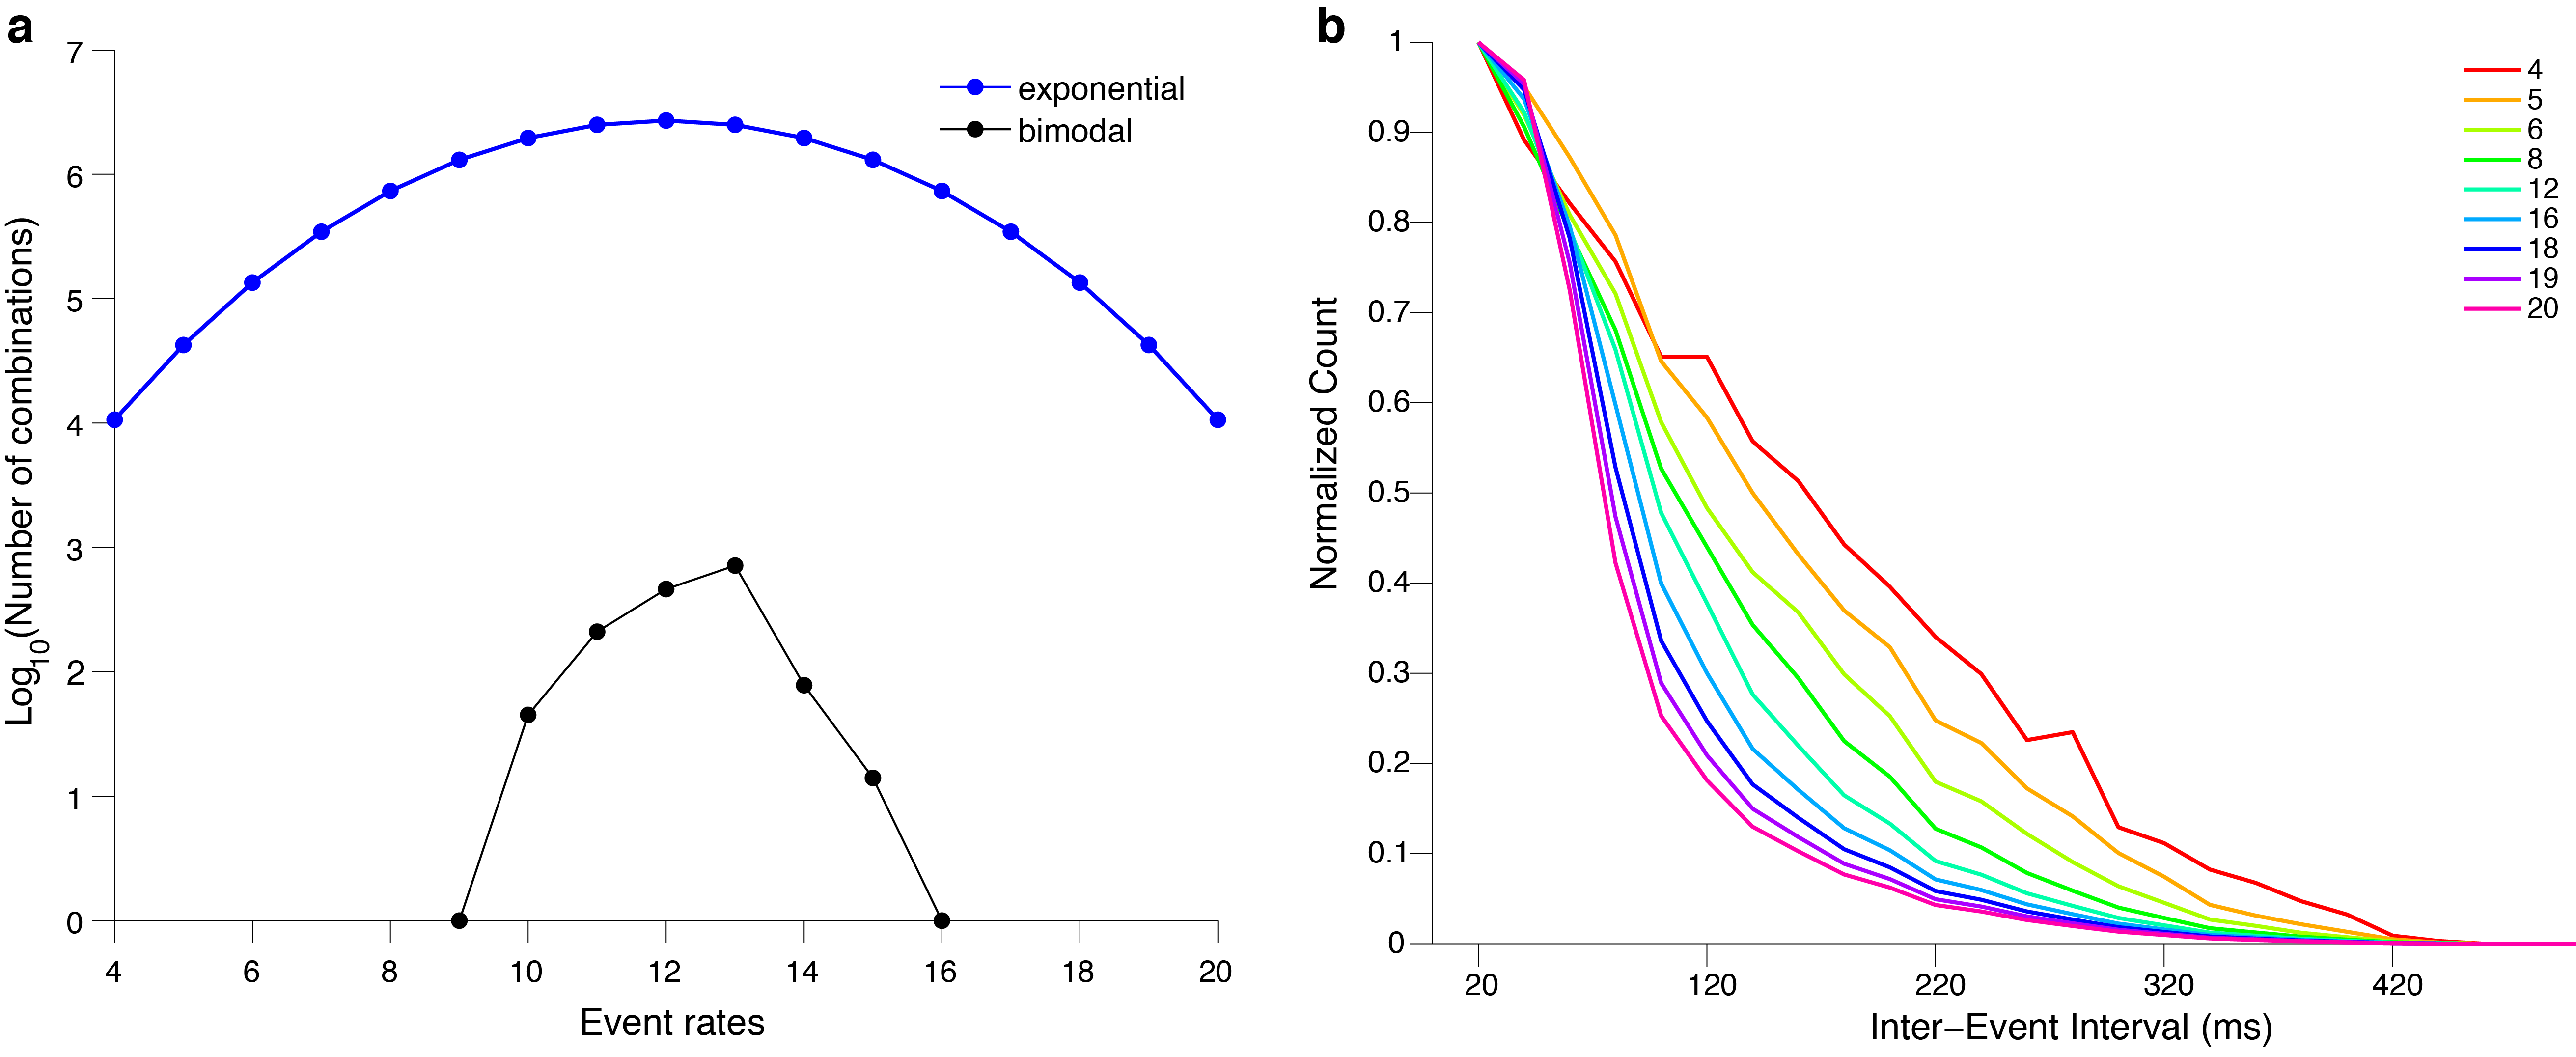
\includegraphics[width=\textwidth] {Figures/chapter2/combo_and_intervals.png}
\caption[Number of possible configurations per flash-rate and histogram of inter-pulse interval]{\textbf{Number of possible configurations per flash rate and histogram of inter-pulse intervals} (a) Comparison of the number of unique pulsatile sequences for each flash rate for the bimodal (black) and exponential interval (blue) pulsatile sequences. (b) Histogram of inter-flash intervals for each flash count in the exponential interval stimulus.}
  \label{fig:combo}\label{fig:stimulusprop}
\end{figure}
%----------------------------------------------------------------------
%----------------------------------------------------------------------
\section{Task Structure}
The behavioral task was performed in a three-port choice box \parencite{Uchida2003}. Mice were trained to self-initiate trials by poking into the center port and maintaining fixation within the center port for up to 1100 ms, while the visual stimulus played (Figure \ref{fig:taskstructure}). At the end of the wait period, an auditory go cue was delivered to inform the subject to make a response. The mice were trained to respond to the right-hand port if the number of flashes exceeded 12 flashes/s (high-rate), and to the left-hand port if the number of flashes was less than 12 flashes/s (low-rate). Mice were given a liquid reward (2-4 $\mu$L of water) for correct responses. Incorrect responses and breaks in center-port fixation were punished with a timeout period of 2-4s, in which the mouse was not allowed to initiate a trial. 
\begin{figure}
  \centering
  	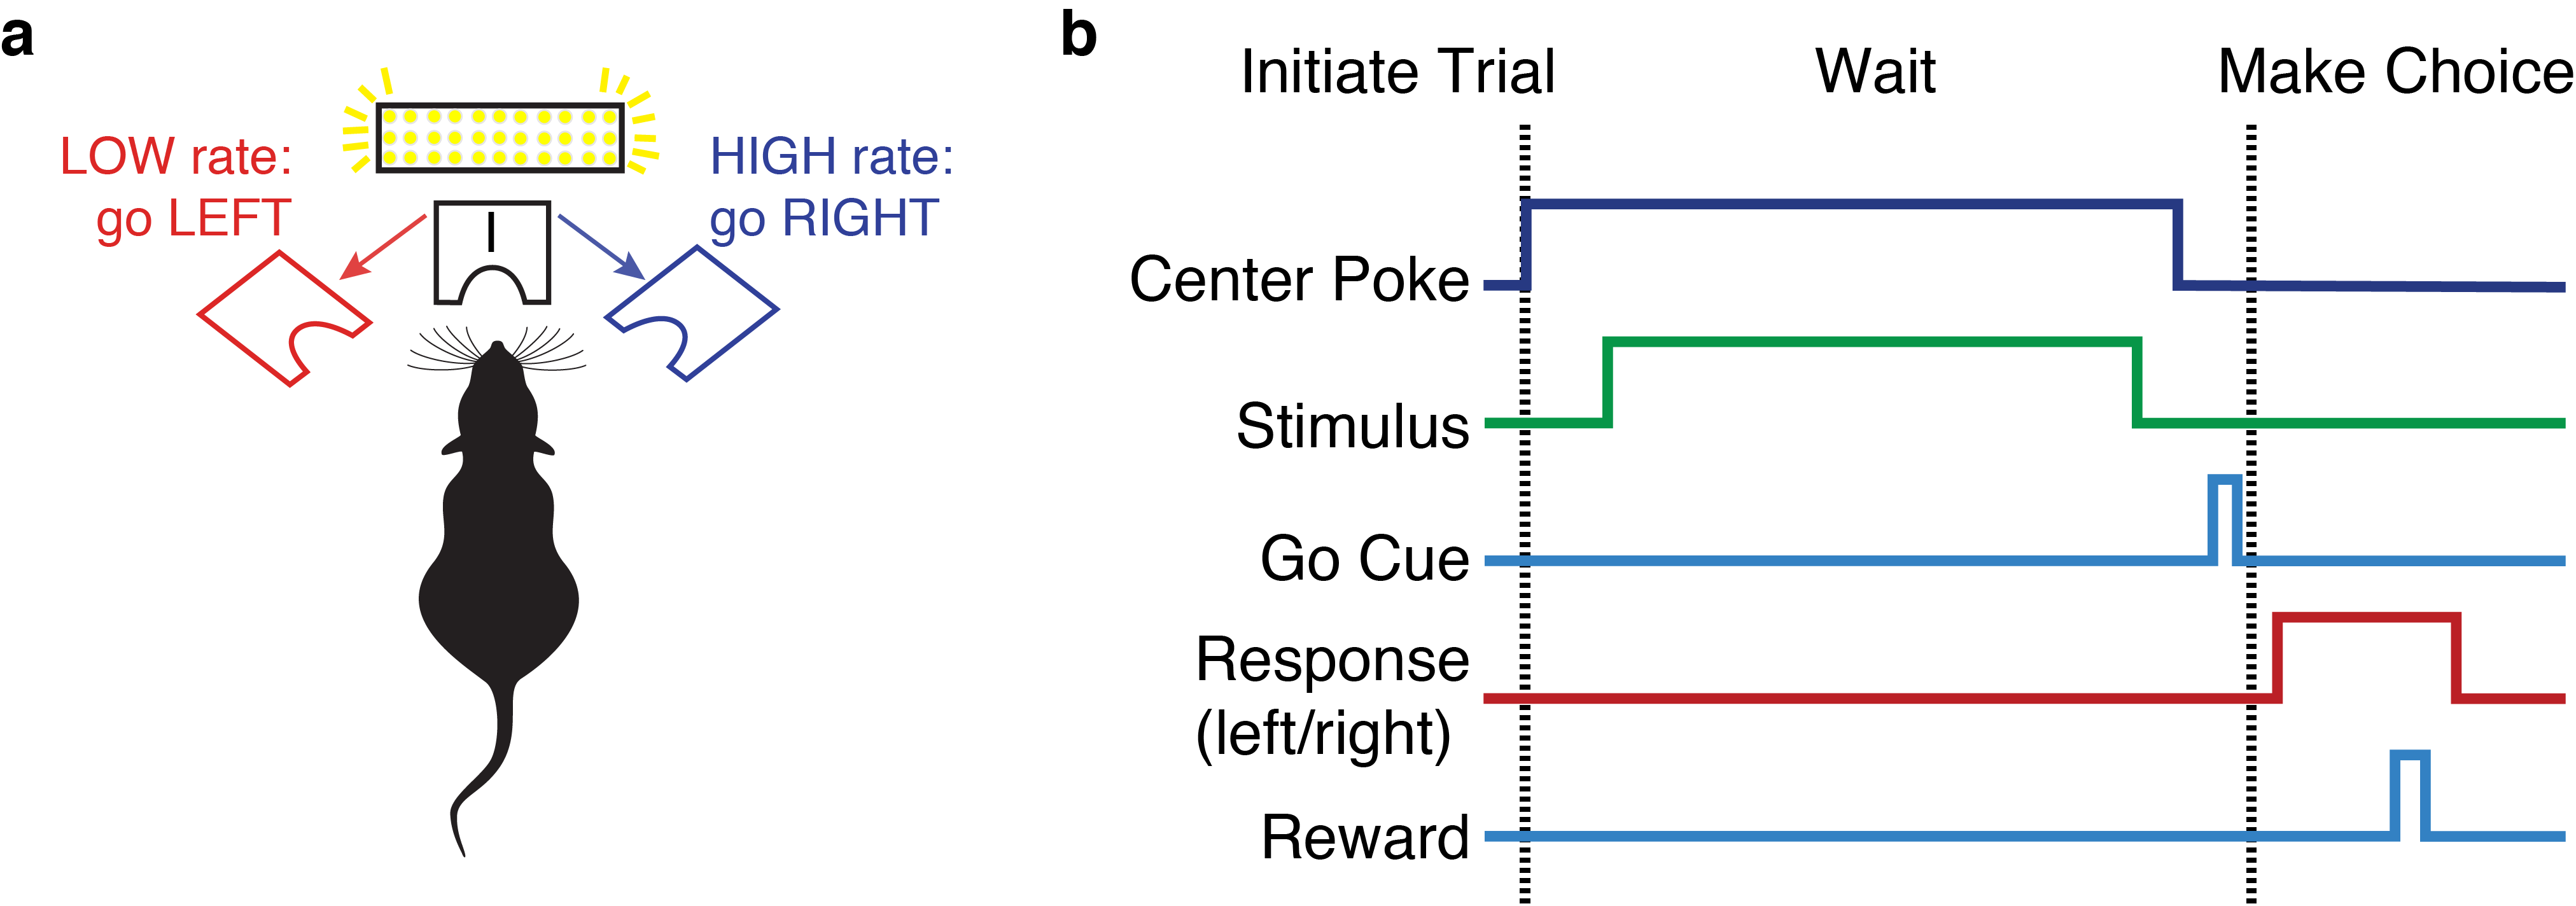
\includegraphics[width=\textwidth]{Figures/chapter2/taskstructure.png}
  \caption[Task Structure]{\textbf{Task Schematic and Trial Structure}. a) Three-port choice task schematic. The mouse initiates trials and stimulus delivery by poking the center port. The mouse responds to whether the stimulus is low-rate (left port) or high-rate (right port). (b) The mouse has to wait at the center port for at least 1100 ms, the stimulus is delivered after a variable delay (10-100ms). At the end of the 1000ms stimulus period, an auditory "Go" tone is played to inform the subject to make a choice. Correct choices to the left or right are rewarded with a small drop of water (2 $\mu$L), incorrect choices earn the subject a 2-3 s timeout.}
   \label{fig:taskstructure}
\end{figure}
%----------------------------------------------------------------------
%----------------------------------------------------------------------
\section{Behavioral Training}
Mice were trained in a semi-automated fashion. The task trial type, stimulus delivery, reward/punishment delivery, and the subjects' responses on each trial were determined and/or recorded by a finite state machine running on an Arduino-based system (Bpod, SanWorks LLC). The subjects' performance was  monitored during each session and occasional intervention was required to shape the behavior, including countering severe side biases or increasing/decreasing the difficulty levels. \par 
Mice performed several hundreds of trials per session (Figure \ref{fig:numTrials}) and acquired the easiest level of the task in less than 20 sessions or 10,000 trials (Figure \ref{fig:pcorrect}). Behavioral training typically lasted for 2-3 months depending on the mice. The mice were trained daily (5 days/week) for up to 2 hours per session.\par 
\begin{figure}
  \centering
  	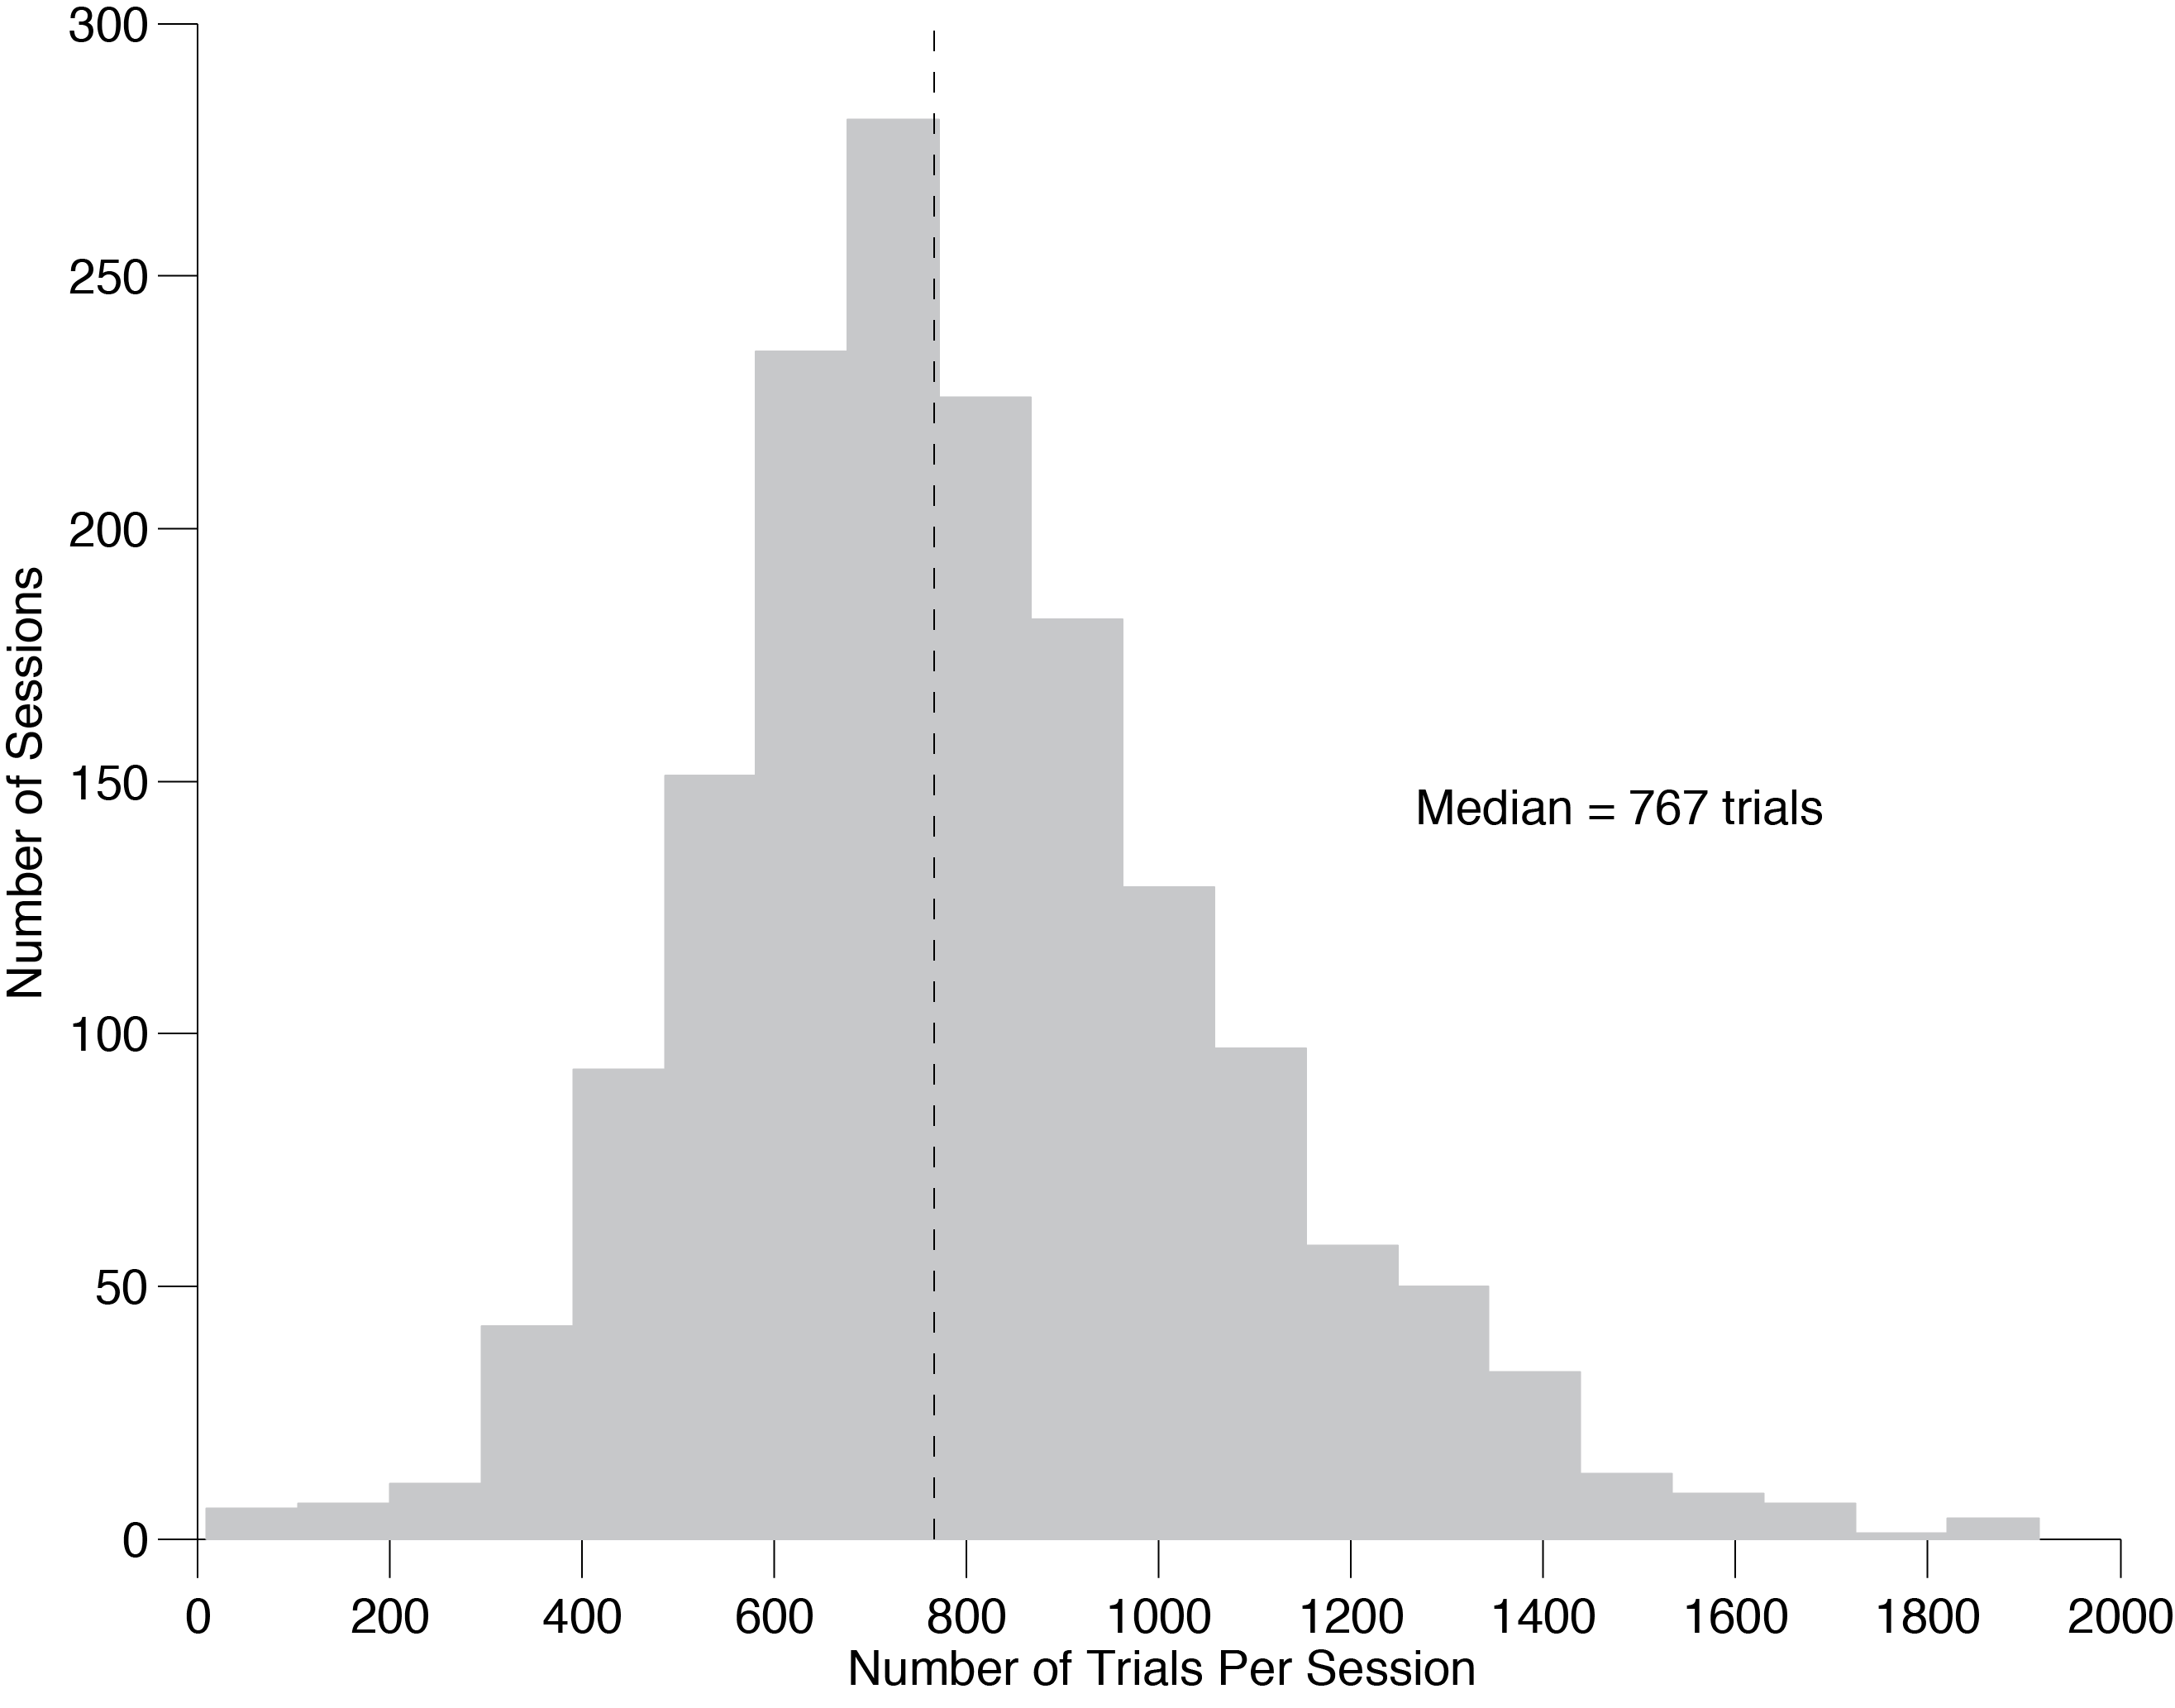
\includegraphics[width=\textwidth]{Figures/chapter2/NumTrialsPerSessions24mice.png}
  \caption[Number of Trials Per Session]{\textbf{Number of Trials Per Session}. Mice performed hundreds of trials per session. n = 24 mice.}
   \label{fig:numTrials}
\end{figure}

The first stage of training was to teach the mice to wait at the center port for at least 1100 ms. This was done by gradually increasing the minimum required wait duration from 25 to 1100ms, by an increment of 0.1 ms on every trial. With this approach, it took the mice about 10-12 sessions to learn to wait for at least 1000 ms (Figure \ref{fig:completeRate} a). During this phase, mice were not rewarded for making the correct association between the stimulus and response port; rather on each trial, a random port (left or right) was chosen as the reward port and a liquid reward was delivered to the port. I found that the number of sessions it took the mice to learn center fixation can be reduced significantly (by a factor of 5), by additionally rewarding the mice at the center port (0.5 $\mu$L) each time they waited the minimum required center wait duration (Figure \ref{fig:completeRate} c). Trials in which the mouse waited the minimum required duration at the center port we refer to as completed trials. Mice rewarded at the center port achieved a completion rate above 90\% compared to mice not rewarded at the center port.\par
%Learning rate multiple mice
\begin{figure}
  \centering
  	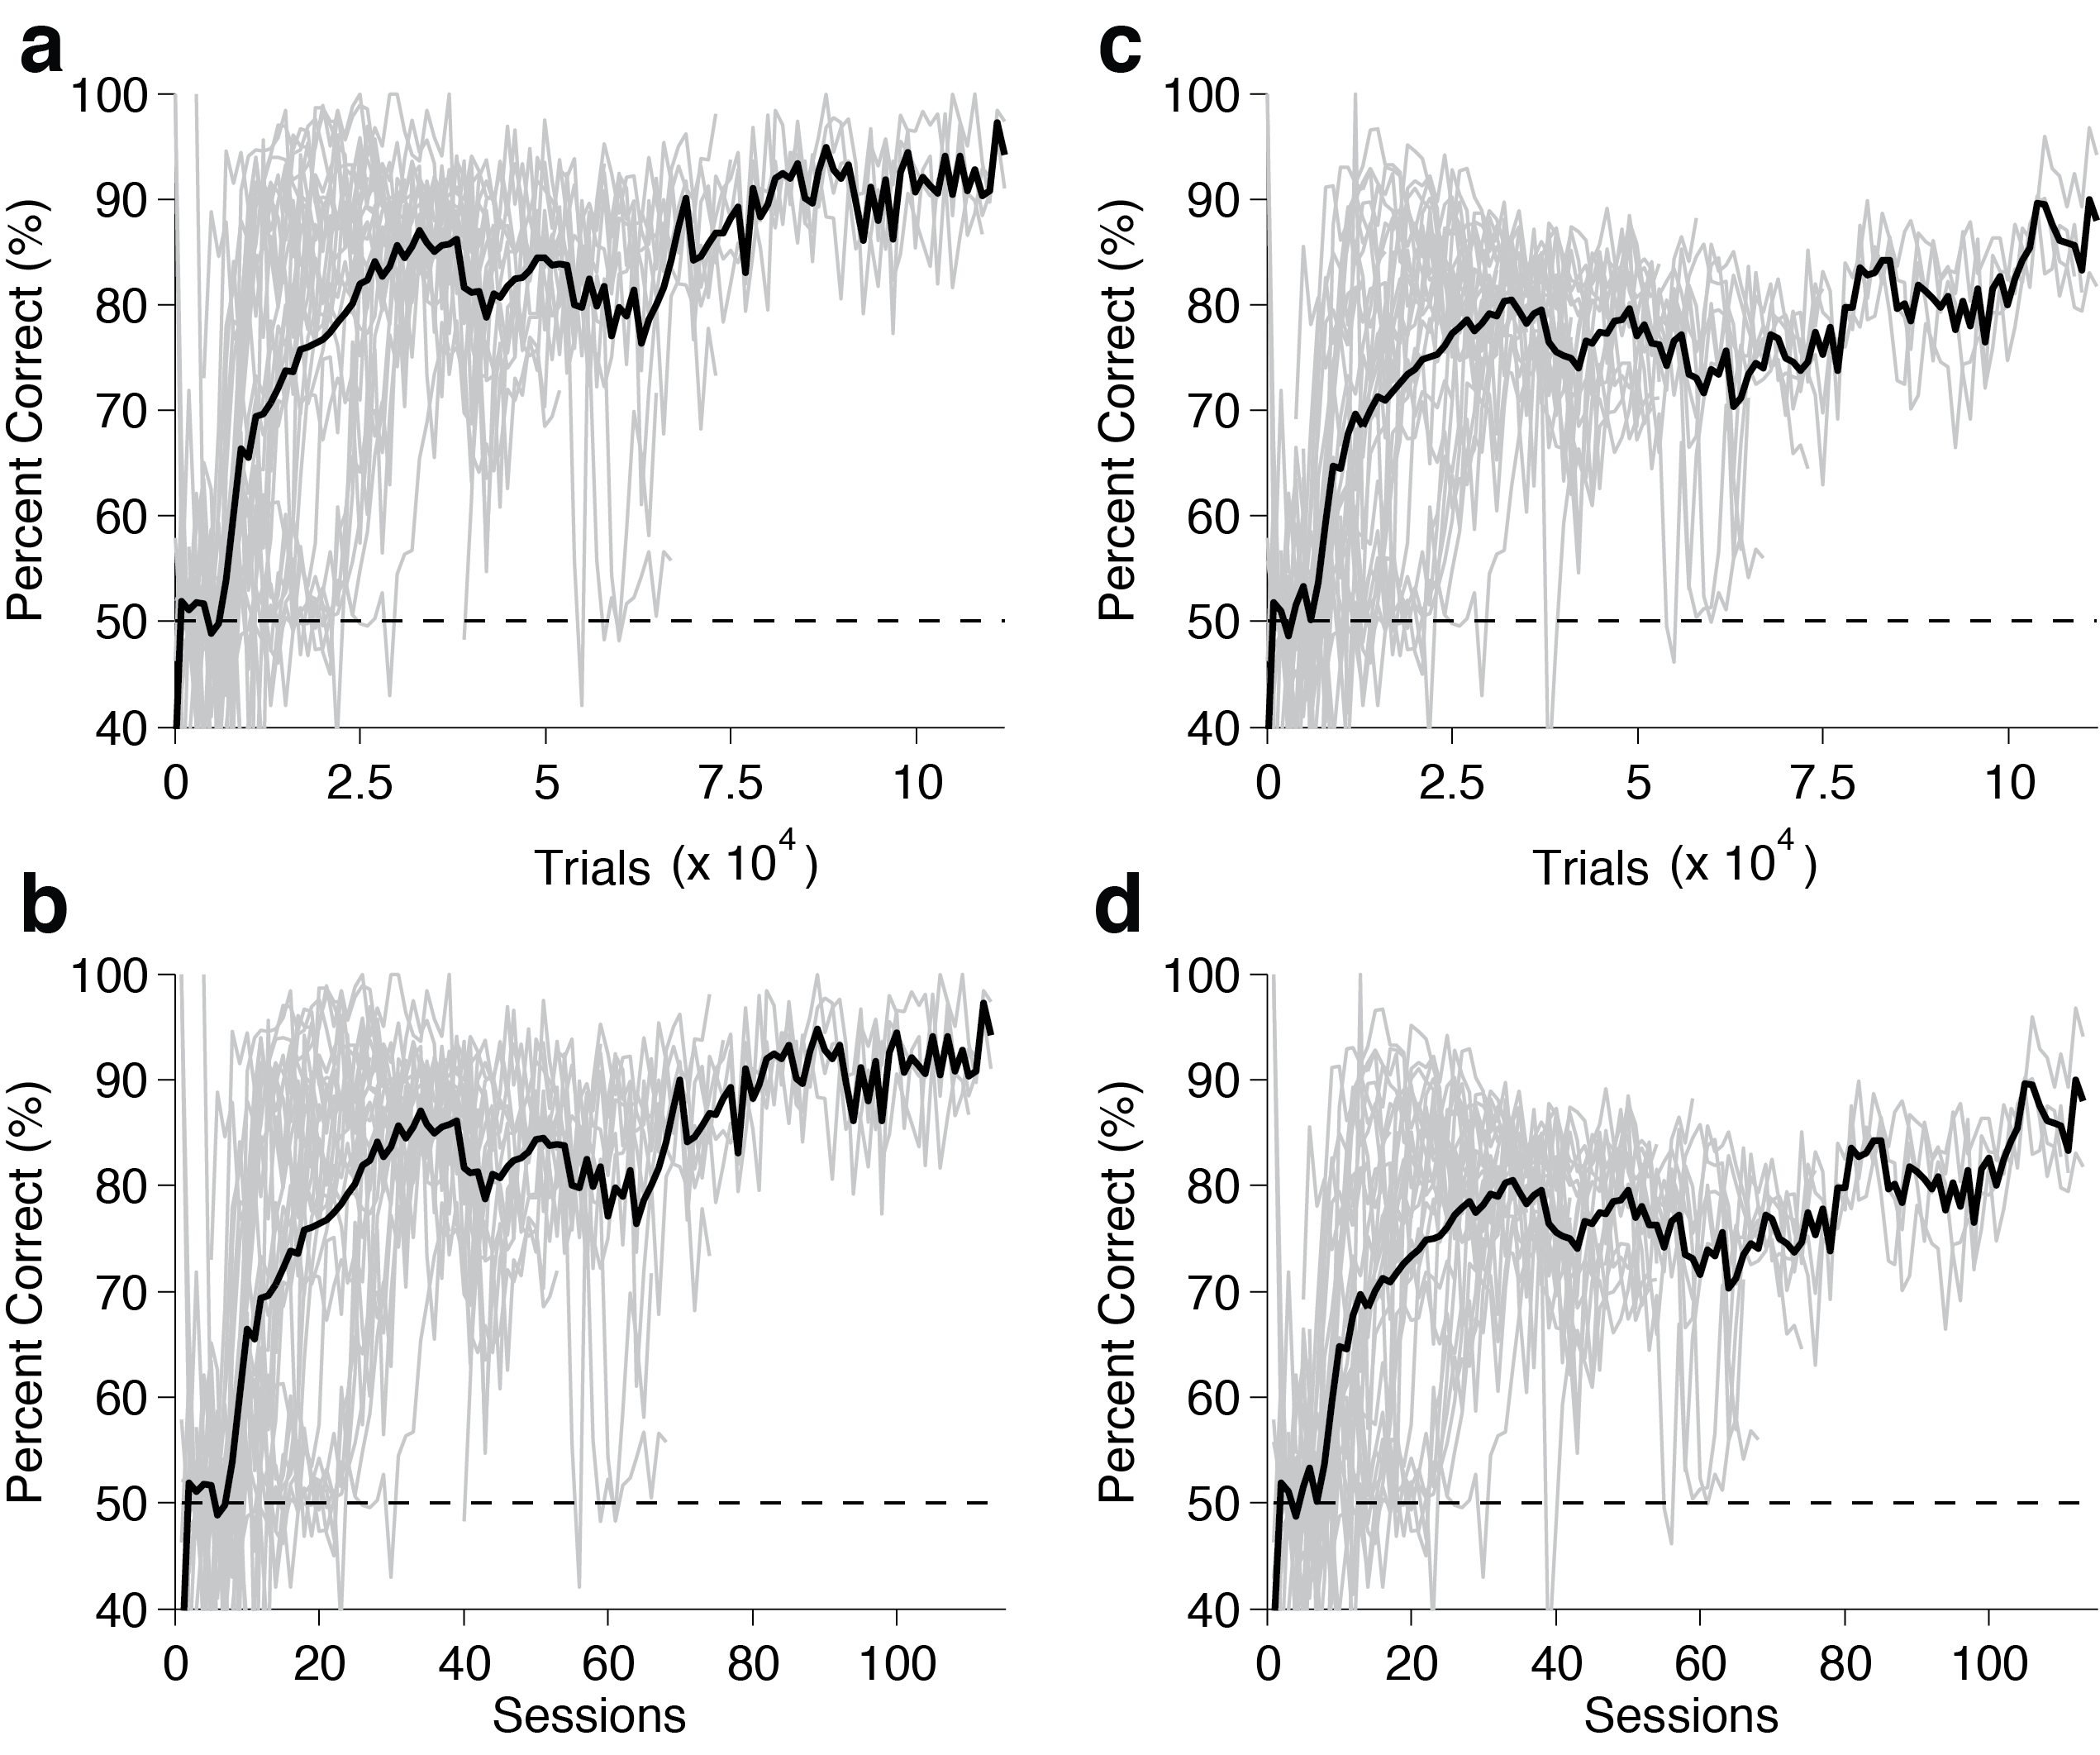
\includegraphics[width=\textwidth]{Figures/chapter2/percentCorrectAllMice.png}
  \caption[Learning Rate]{\textbf{Learning Rate of Multiple Mice.} (a) Percent correct on easiest stimulus conditions (4 and 20 flashes/s) and (c) Percent correct on all stimulus conditions plotted across trials and sessions. Gray traces are individual mice. Black trace, average across mice (n = 24 mice).}
   \label{fig:pcorrect}
\end{figure}
In the second stage of training mice were trained to associate high-rate flashes (>12 flashes/s) with the right-hand port and low-rate flashes (< 12 flashes/s) with the left-hand port. For some mice, the contingency was reversed, such that high-rate flashes were rewarded at the left-hand port and low-rate flashes were rewarded at the right-hand port. The mice learned this phase by trial and error. They were rewarded for making the correct association and punished with a time-out period for incorrect responses. Trials with flash rates of 12 flashes/s were randomly rewarded on the left or right hand port. During this phase, mice typically developed strong side biases, for instance always going to the right-hand port. Depending on the severity of the bias, one of several strategies for countering the bias was used including adjusting the reward volumes/ratio on the left vs right port, adjusting the proportion of left vs right trials, and/or physically blocking access to the biased port. We also made use of custom written antibias software in the lab to handle minor cases of bias. \par 
\begin{figure}
  \centering
  	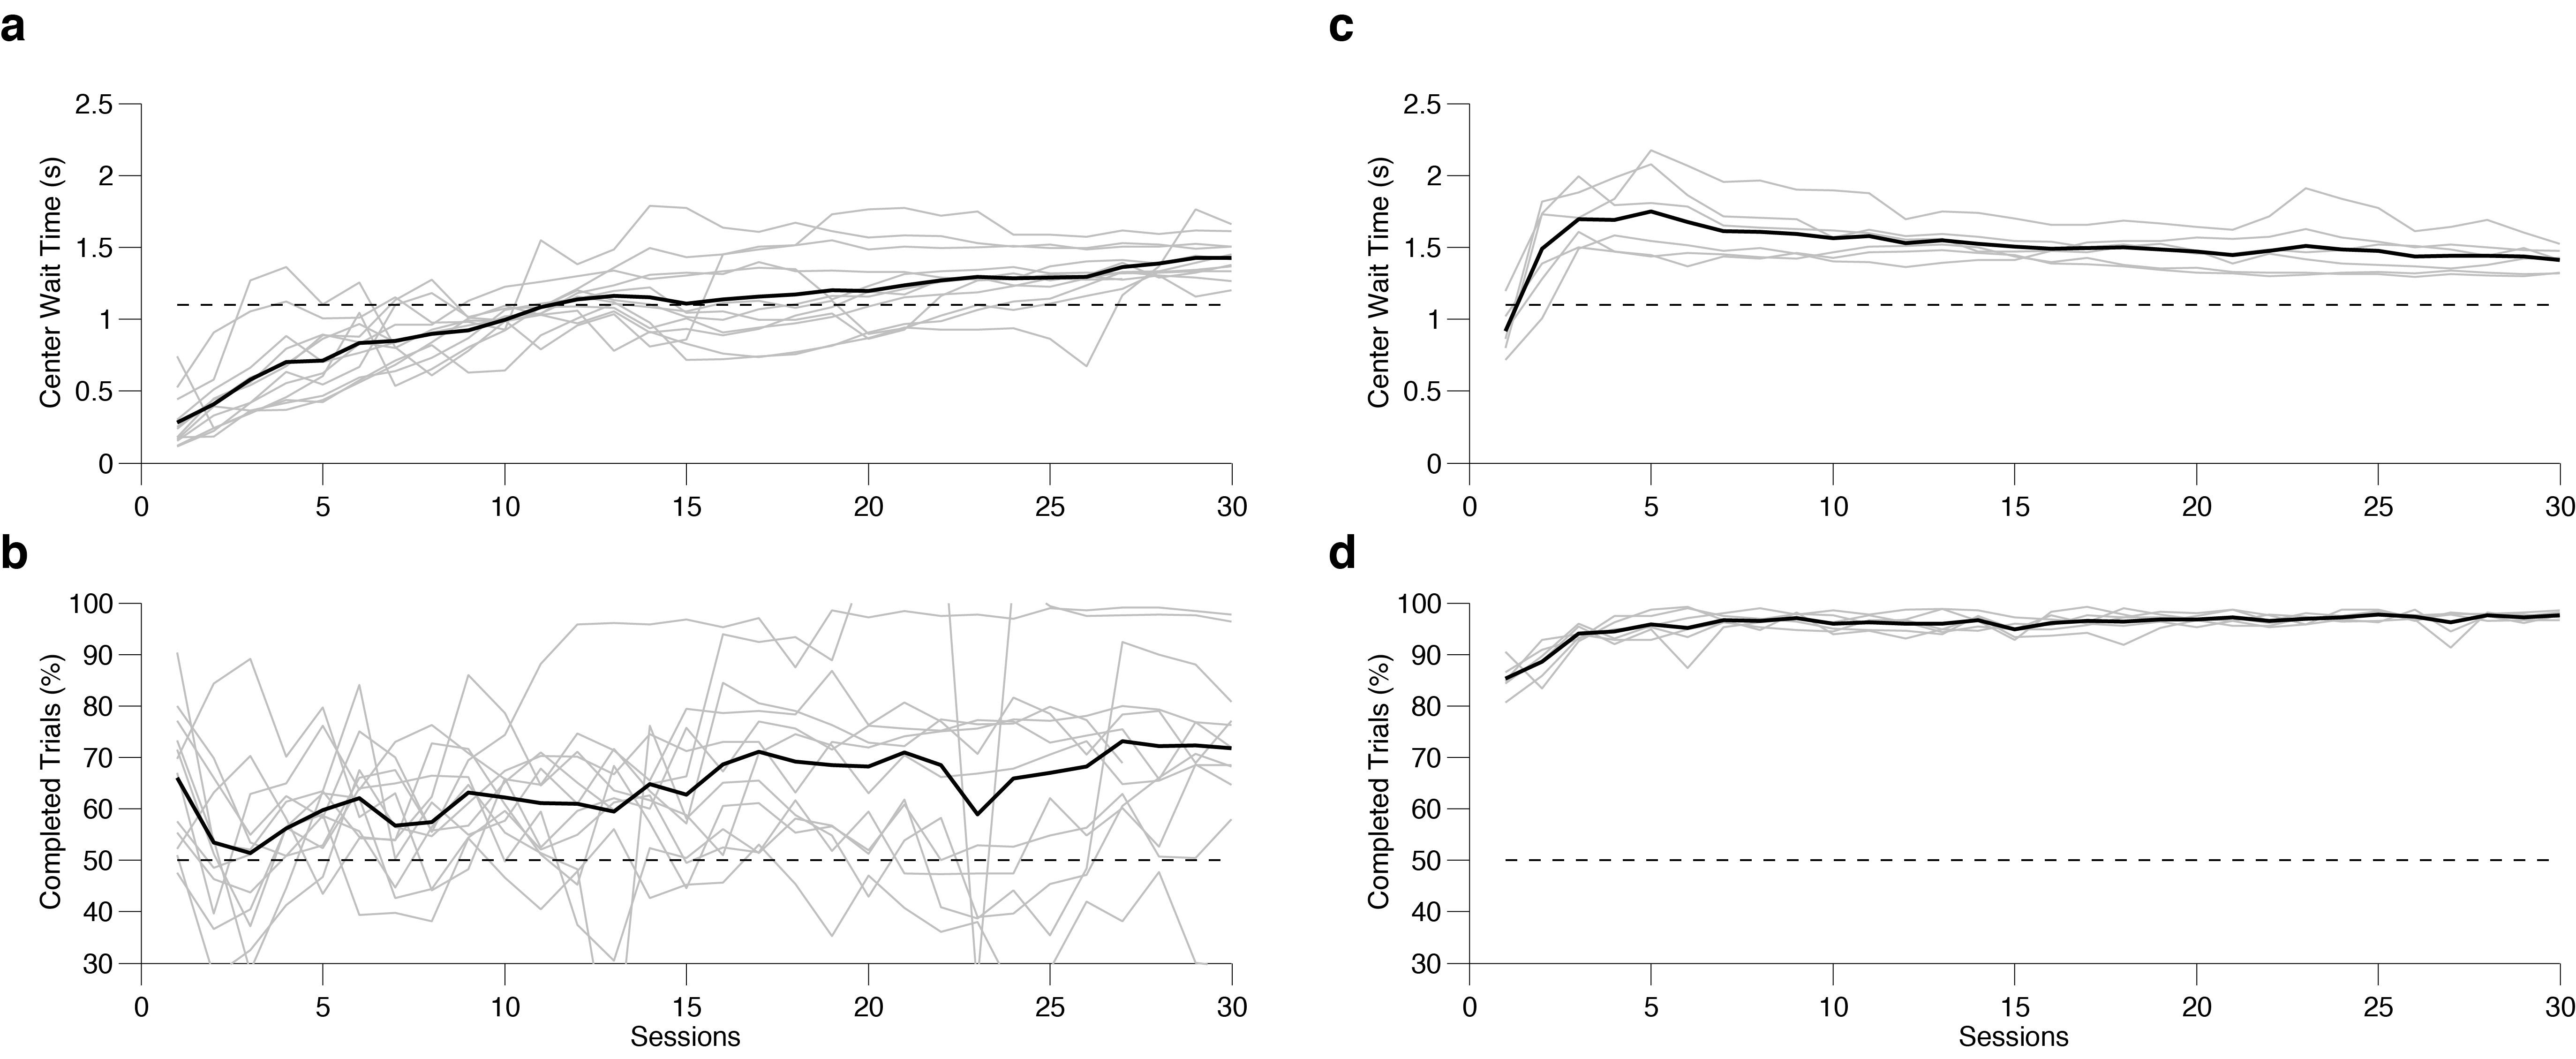
\includegraphics[width=\textwidth]{Figures/chapter2/CenterWaitTimeandCompletionRateComparison.png}
  \caption[Median Center Wait Duration and Trial Completion Rate]{\textbf{Median Center Fixation and Trial Completion Rate.} Comparison between (a,b) Mice that were not rewarded at the center (n = 12) (c-d) Mice rewarded at the center port (n = 6). Gray traces, individual mice. Black trace, average mouse.}
   \label{fig:completeRate}
\end{figure}
In the first two phases, the mice were presented with the easy flash rates at the extremes of the stimulus range (4, 5, 19 \& 20 flashes/s). As the mice improved in performance,  flash rates closer to the category boundary (12 flashes/s) were gradually introduced. For symmetry, rates were introduced in pairs (eg. 4 \& 20, 5 \& 19, 6 \& 18, 8 \& 18 etc). Mice initially had trouble achieving high performance with only 1000 ms of stimulus. To help them during training, the stimulus was extended beyond 1000 ms by repeating the same stimulus sequence for an additional 1000 ms. The extended portion of the stimulus was gradually reduced over the course of training. A fully trained mouse experiences at least 6 pairs of flash rates and waits for at least 1100 ms at the center port. This criteria typically takes at least 1 month to achieve. In 2-3 months, trained mice can experience the entire range of flash rates without the extended stimulus.
%--------------------------------------------------------------------
\section{Psychometric Performance}
The subject's performance on the task is quantified with a psychometric function (Figure \ref{fig:pmfs}). The psychometric function is a quantitative description of the relationship between stimulus features and the subject's choices on a psychophysical paradigm and is used as an inference model of the underlying perceptual mechanism used to perform the discrimination task. While the true underlying function used by the subjects to solve the task is unknown \parencite{Kingdom2010}, typically psychometric curves are generated by fitting a sigmoidal function such as the logistic function or cumulative Gaussian \parencite{Wichmann2001}. In general, for the data in this thesis, we fit the psychometric curve using either logistic or cumulative Gaussian function. Both functions fit the data similarly.\par 
For the visual pulses discrimination task, the general form of the psychometric function defines the probability (\emph{$p_h$}) that the subject chooses the port associated with high flash rates as:
\begin{equation}
	\centering
	p_h = \gamma + (1-\gamma - \lambda)F(x;\alpha,\beta)
\end{equation}
where $\gamma$ and $\lambda$ are the lower and upper asymptote of the psychometric function, which parameterize the guess rate and lapse rate, respectively; \emph{F} is a sigmoidal function, in our case either the logistic function or cumulative Normal distribution; \emph{x} is the event rate i.e. the number of flashes presented during the one second stimulus period; $\alpha$ parameterizes the horizontal shift or bias of the psychometric function and $\beta$ describes the slope or inverse sensitivity. The steeper the slope ($\beta$) the better the psychophysical performance. The psychometric function \emph{F(x;$\alpha$,$\beta$)} for a cumulative Gaussian distribution is defined as: 
\begin{equation}
	\centering
	F(x;\alpha,\beta) = \frac{\beta}{\sqrt[]{2\pi}} \int_{-\infty}^{x} \exp(\frac{-\beta^{2}(x-\alpha)^{2}}{2})
   \label{eq:normalpmf}
\end{equation}
where $\beta$ is the slope of the psychometric function and also the inverse of the width of the Gaussian (i.e. $\sigma$). 
\begin{figure}
  \centering
  	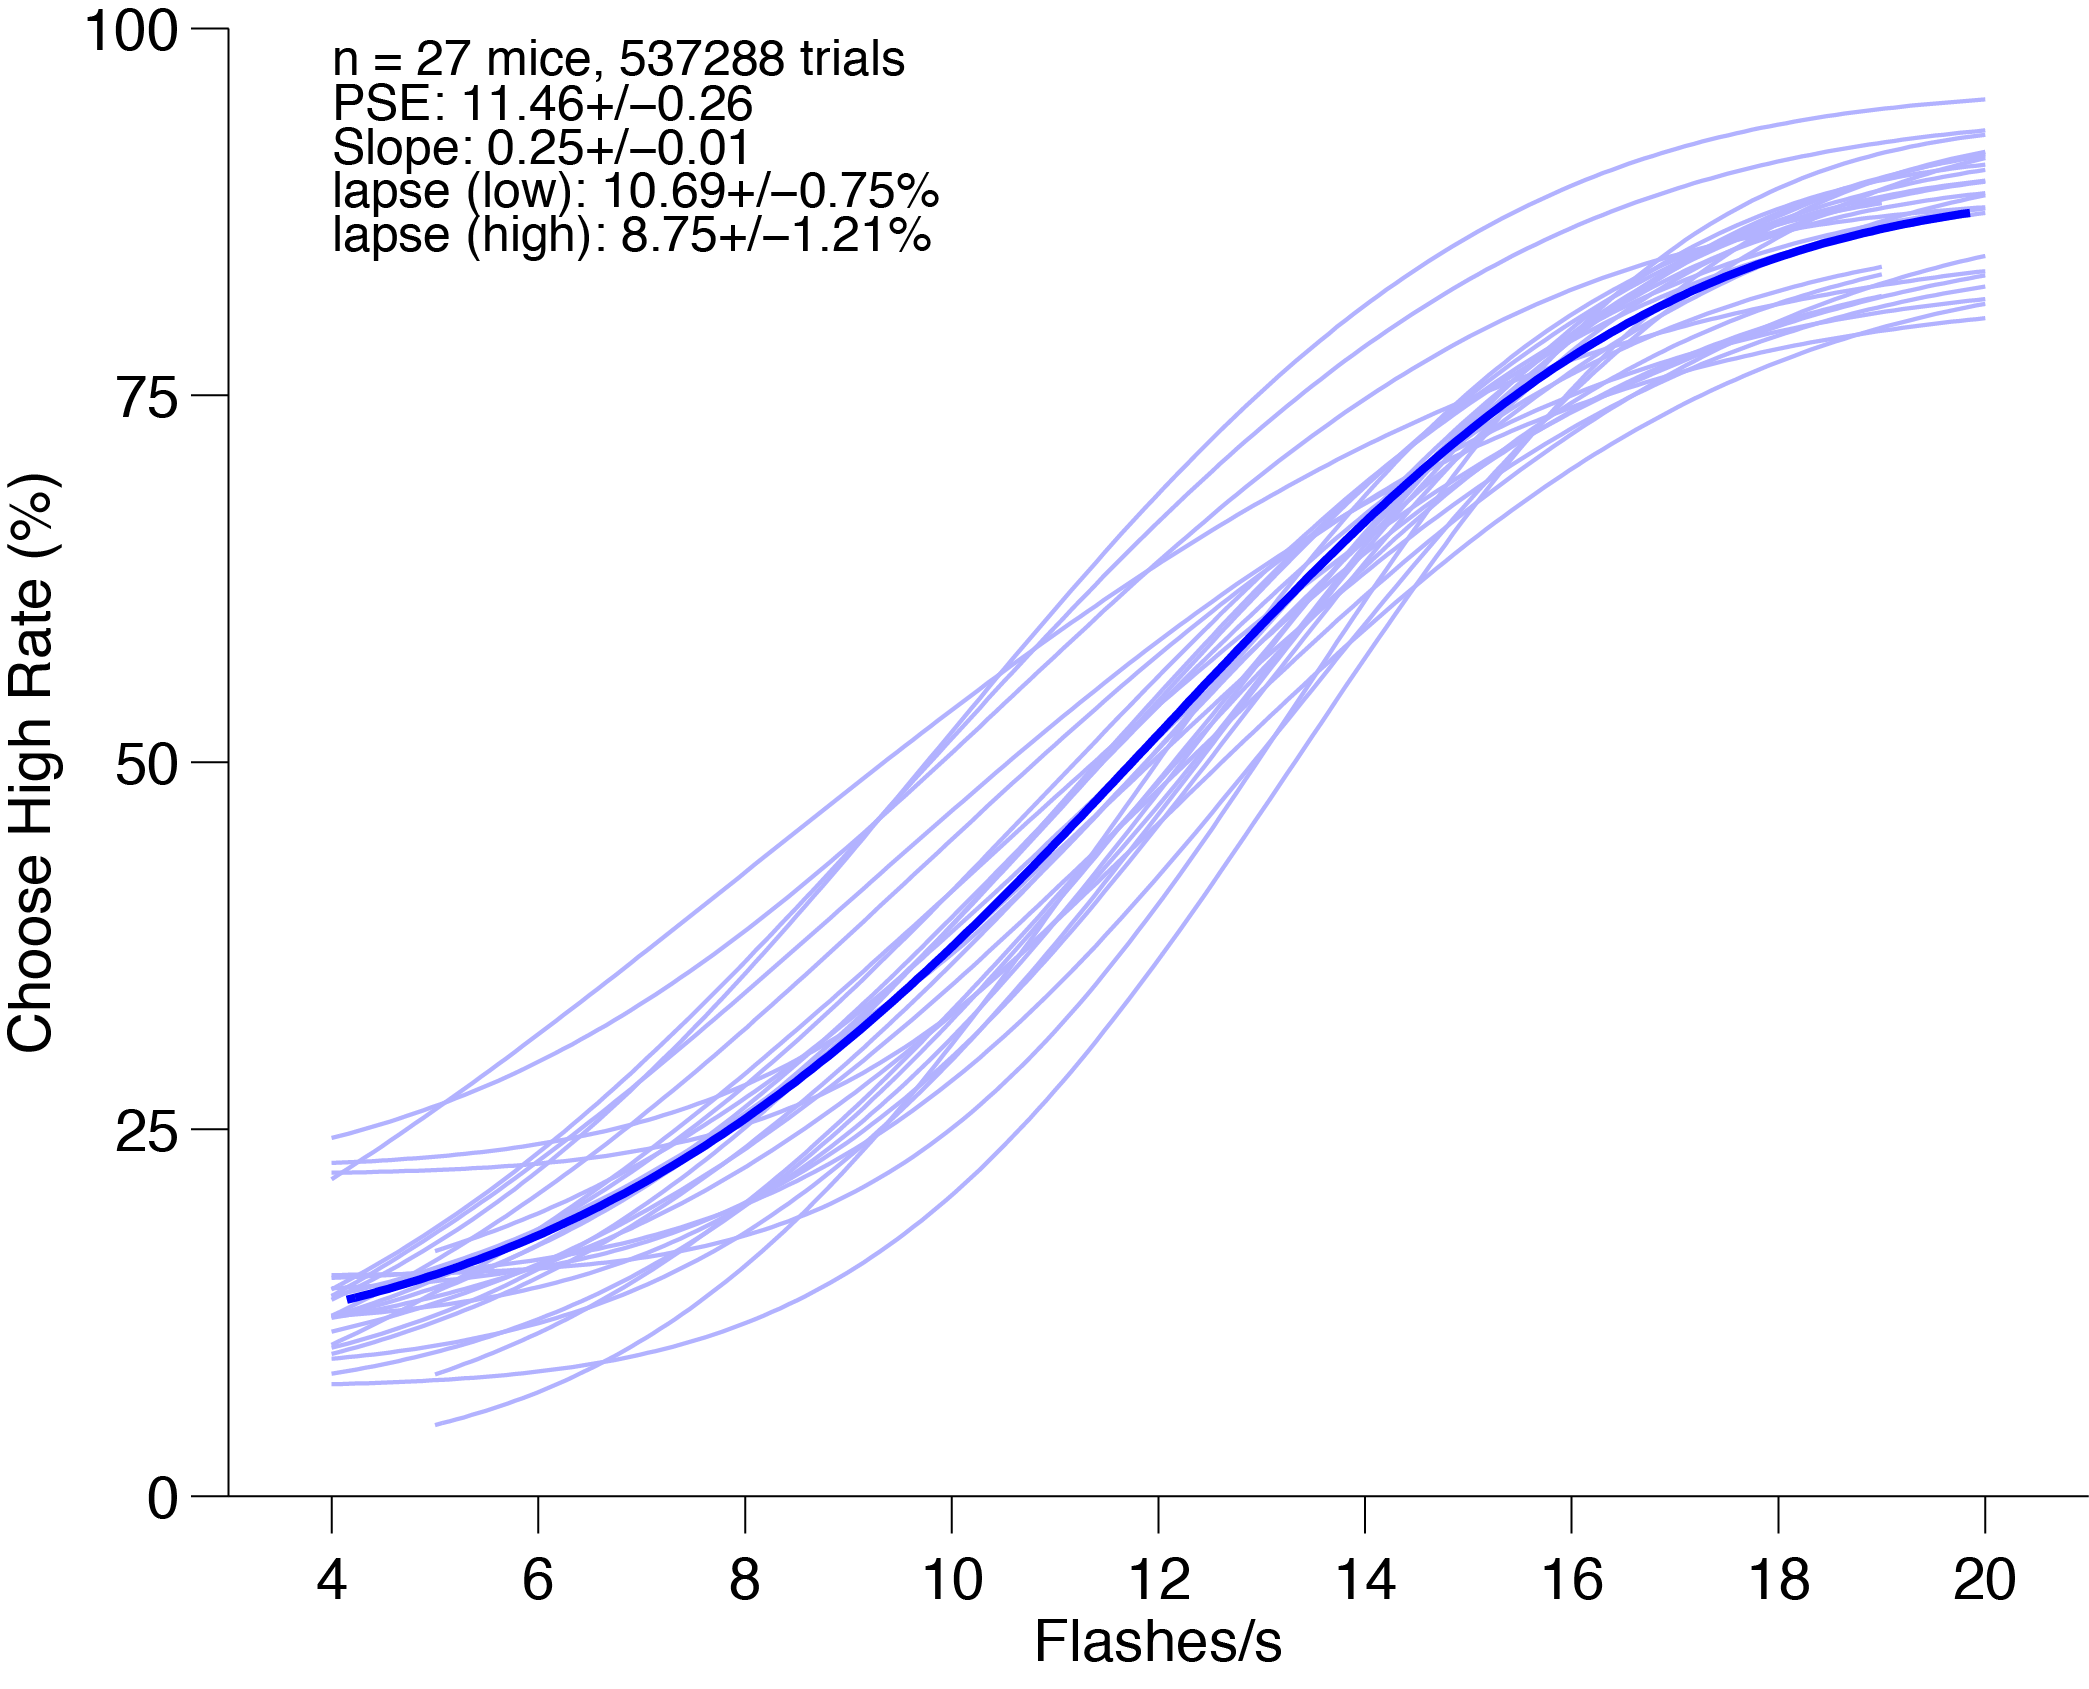
\includegraphics[width=\textwidth]{Figures/chapter2/PMF_pal_27_mice.png}
  \caption[Psychometric Functions]{\textbf{Psychometric Function} fits for individual mice (light blue trace) and average mouse (dark blue). n = 27 mice, across multiple sessions. The psychometric functions were fit with a 4-parameter cumulative Normal distribution to individually fit the intercept, slope, lapse rate and guess rate.}   
   \label{fig:pmfs}
\end{figure}
%----------------------------------------------------------------
\section{Psychophysical Reverse Correlation}
An ideal solution to the task is to sum all the flashes presented during the fixed stimulus presentation period, i.e. apply an equal weight to each incoming flash until the go cue. However, it's not clear whether the mice trained on this task adopted such strategy. For example, the mouse could adopt a strategy where it only pays attention to the first (or second) half of the stimulus. Attention to the flash events early in the sequence would reflect an impulsive strategy, whereas attention to flash events later in the sequence would reflect a leaky or forgetful strategy.\par 
Psychophysical reverse correlation analysis, also known as choice-triggered average, is used to measure the psychophysical kernel of the mice trained on the visual pulses task. There are a number of published methods for performing psychophysical reverse correlation analysis \parencite{Huk2005,Nienborg2007,Raposo2012a,Brunton2013,Katz2016}; however, a simple approach is to use logistic regression  \parencite{Huk2005,Znamenskiy2013,Katz2016}. In the logistic regression approach, the design matrix (i.e. regressors) consists of the pulsatile stimulus sequence for each trial, with 1's to indicate whether a flash occurred in a time bin. The goal is to estimate the weights (coefficients) associated with each time bin.\par 

The logistic regression function for estimating the weights associated with each moment of the stimulus can be written as:
\begin{equation}
	\centering
	\ln(\frac{p_h}{1-p_h}) = \beta_0 + \sum_{i=1}^{N=25} \beta_iI
\end{equation}
where $p_h$ is the probability of choosing the high-rate port, $\emph{I}$ is an indicator variable for whether or not a flash pulse occurred in time bin $\emph{i}$, and $\emph{N}$ is the number of time bins. The coefficients $\beta_0$,...,$\beta_N$ are estimated with the MATLAB function $\emph{glmfit}$. \par 
The logistic reverse correlation approach reveals how each incoming flash, on average, influences the subject's choice. Across mice (Figure \ref{fig:allkernels}), the entire sequence of flashes was informative, as indicated by non-zero regression weights. Also, flashes presented earlier in the sequence appeared to be more informative of the choice than later flashes, on average. The mice appear to make snap judgments about the stimulus sequence, reflecting an impulsive integration strategy. Although the shape of the psychophysical kernel observed in the mice are similar to those observed in nonhuman primate subjects \parencite{Katz2016}, they differ from kernels that have been observed in rats (Figure \ref{fig:ratkernel}) \parencite{Raposo2012,Brunton2013,Scott2015SourcesRats}. In rats, the psychophysical kernels are mostly flat, reflecting an average integration in which evidence is integrated uniformly over time. 
\begin{figure}
  \centering
  	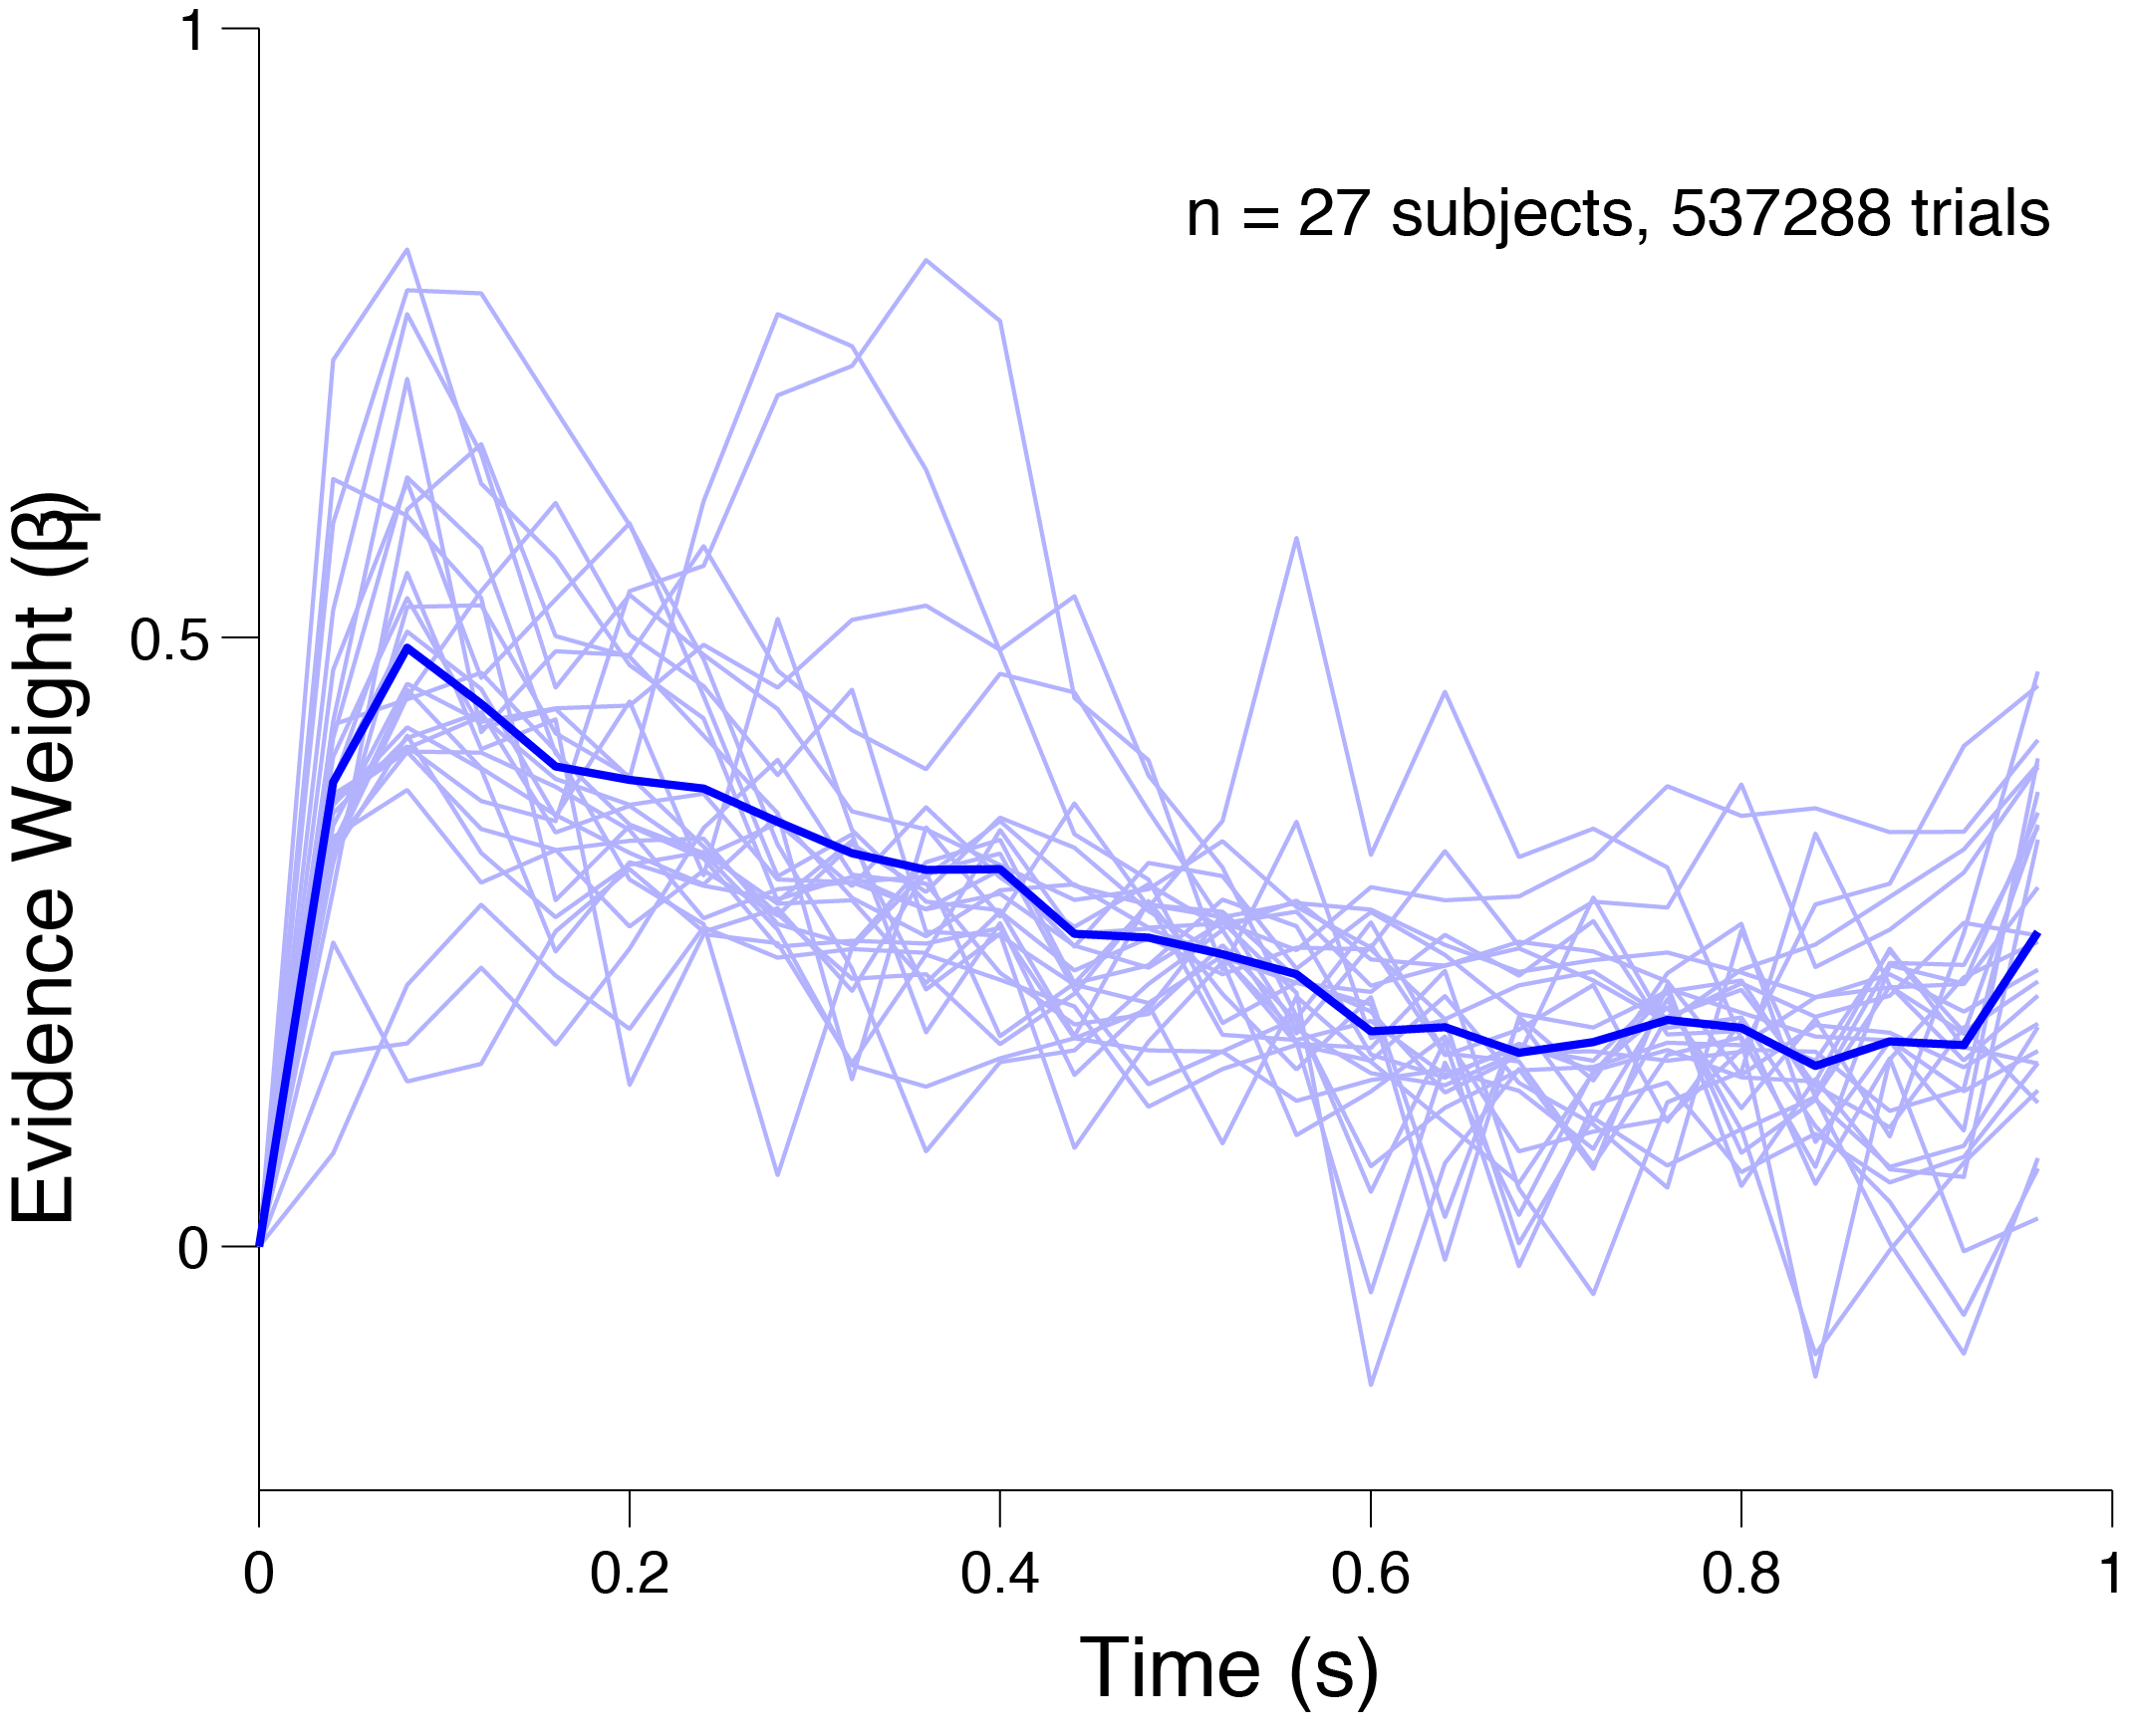
\includegraphics[width=\textwidth]{Figures/chapter2/psychKernel_all_mice.png}
  \caption[Psychophysical Kernels ]{\textbf{Psychophysical Kernels} of individual mice (light blue) and average across mice (dark blue).}
   \label{fig:allkernels}
\end{figure}
%----------------------------------------------------------------------------
\section{Brightness Manipulation}
An alternate strategy to solve the visual pulses task is to accumulate photons or brightness over time, such that the decision is based on the final brightness value. This is a valid strategy given that the flash event rate is directly proportionally to the amount of time the LED is on, and therefore the number of photons emitted (or perceived brightness) over time (Figure \ref{fig:brightness_sim_man}). To test whether subjects performing the visual pulses task were sensitive to changes in brightness, I performed two brightness manipulation experiments. In the first manipulation experiment, the flash sequence was made dimmer or brighter randomly on 5\% of trials. The prediction is that subjects using a brightness strategy will tend to report more high-rate choices on trials with brighter pulse sequences, and on dimmer trials report low-rate choices. For comparison, I also tested rats on the same manipulation. Both mice and rats exhibited shifts in the psychometric function consistent with the predictions (Figure \ref{fig:brightness_exp1}). For mice, changes in brightness had a modest effect on the psychometric performance whereas rats were more sensitive to the  brightness perturbation than mice. \par 
A second, more strict, brightness manipulation was to remove the correlation brightness and the flash rate. To do so, the overall brightness of the flash sequence was made proportional to the flash event rate, such that the total brightness over time was the same across flash rates  (Figure \ref{fig:brightness_sim_man}). If the subjects were indeed invariant to the total brightness over time, and instead were counting, this manipulation should not interfere with their performance. However, when the scaled brightness was introduced randomly on 5\% of trials, the performance of both mice and rats were severely affected. \par 
The brightness manipulations revealed that the subjects were not invariant to the brightness. The manipulations do not suggest that the subjects are incapable of using a counting strategy to solve the visual pulses categorization task, especially in the case of the mice. Rather, these experiments reveal that the use of brightness is a valid alternate (or parallel) strategy given that the correlation between the total LED ON time is and the total number of flashes exists in the stimulus (Figure \ref{fig:brightness_sim}). The decreased performance on the second brightness manipulation trials could be explained by the fact that the stimulus is very different from the one on which the subjects were trained. Future efforts could explore whether rodents can be trained on a stimulus similar to Figure \ref{fig:brightness_sim_man}, without the brightness correlation. 

\begin{figure}
  \centering
  	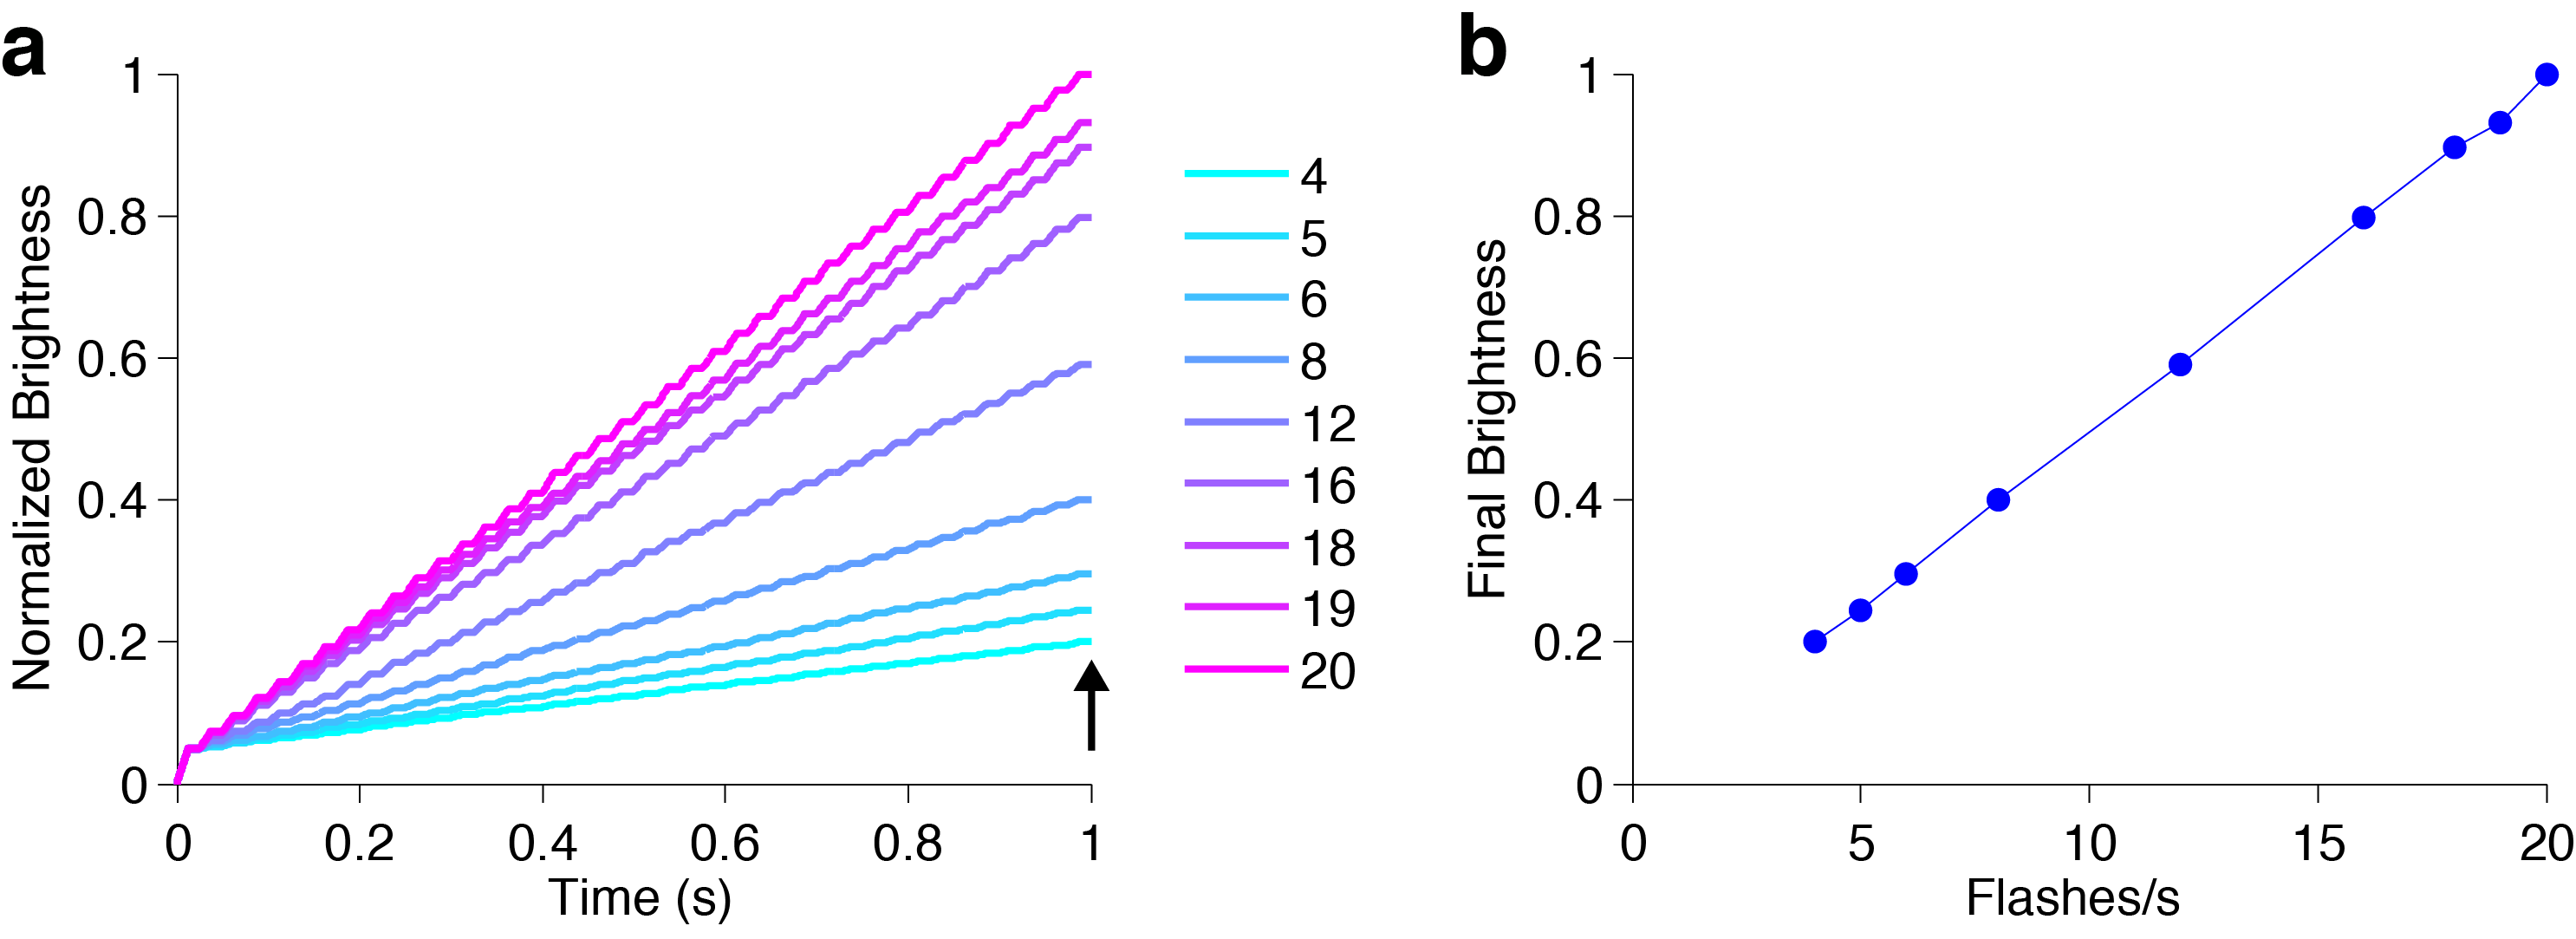
\includegraphics[width=\textwidth]{Figures/chapter2/brightness_simulation_unscaled.png}
  \caption[Flash Rate is Correlated with Brightness Over Time]{\textbf{Trial Flash Rate is Correlated with Brightness Over Time}. (a) Schematic of simulated average brightness (normalized) across time for individual flash rates. Simulated brightness curves computed as the cumulative sum of the flash sequence for a given flash rate. (b) Final simulated brightness value (at arrow in (a)) plotted against flash rate.}
   \label{fig:brightness_sim}
\end{figure}

\begin{figure}
  \centering
  	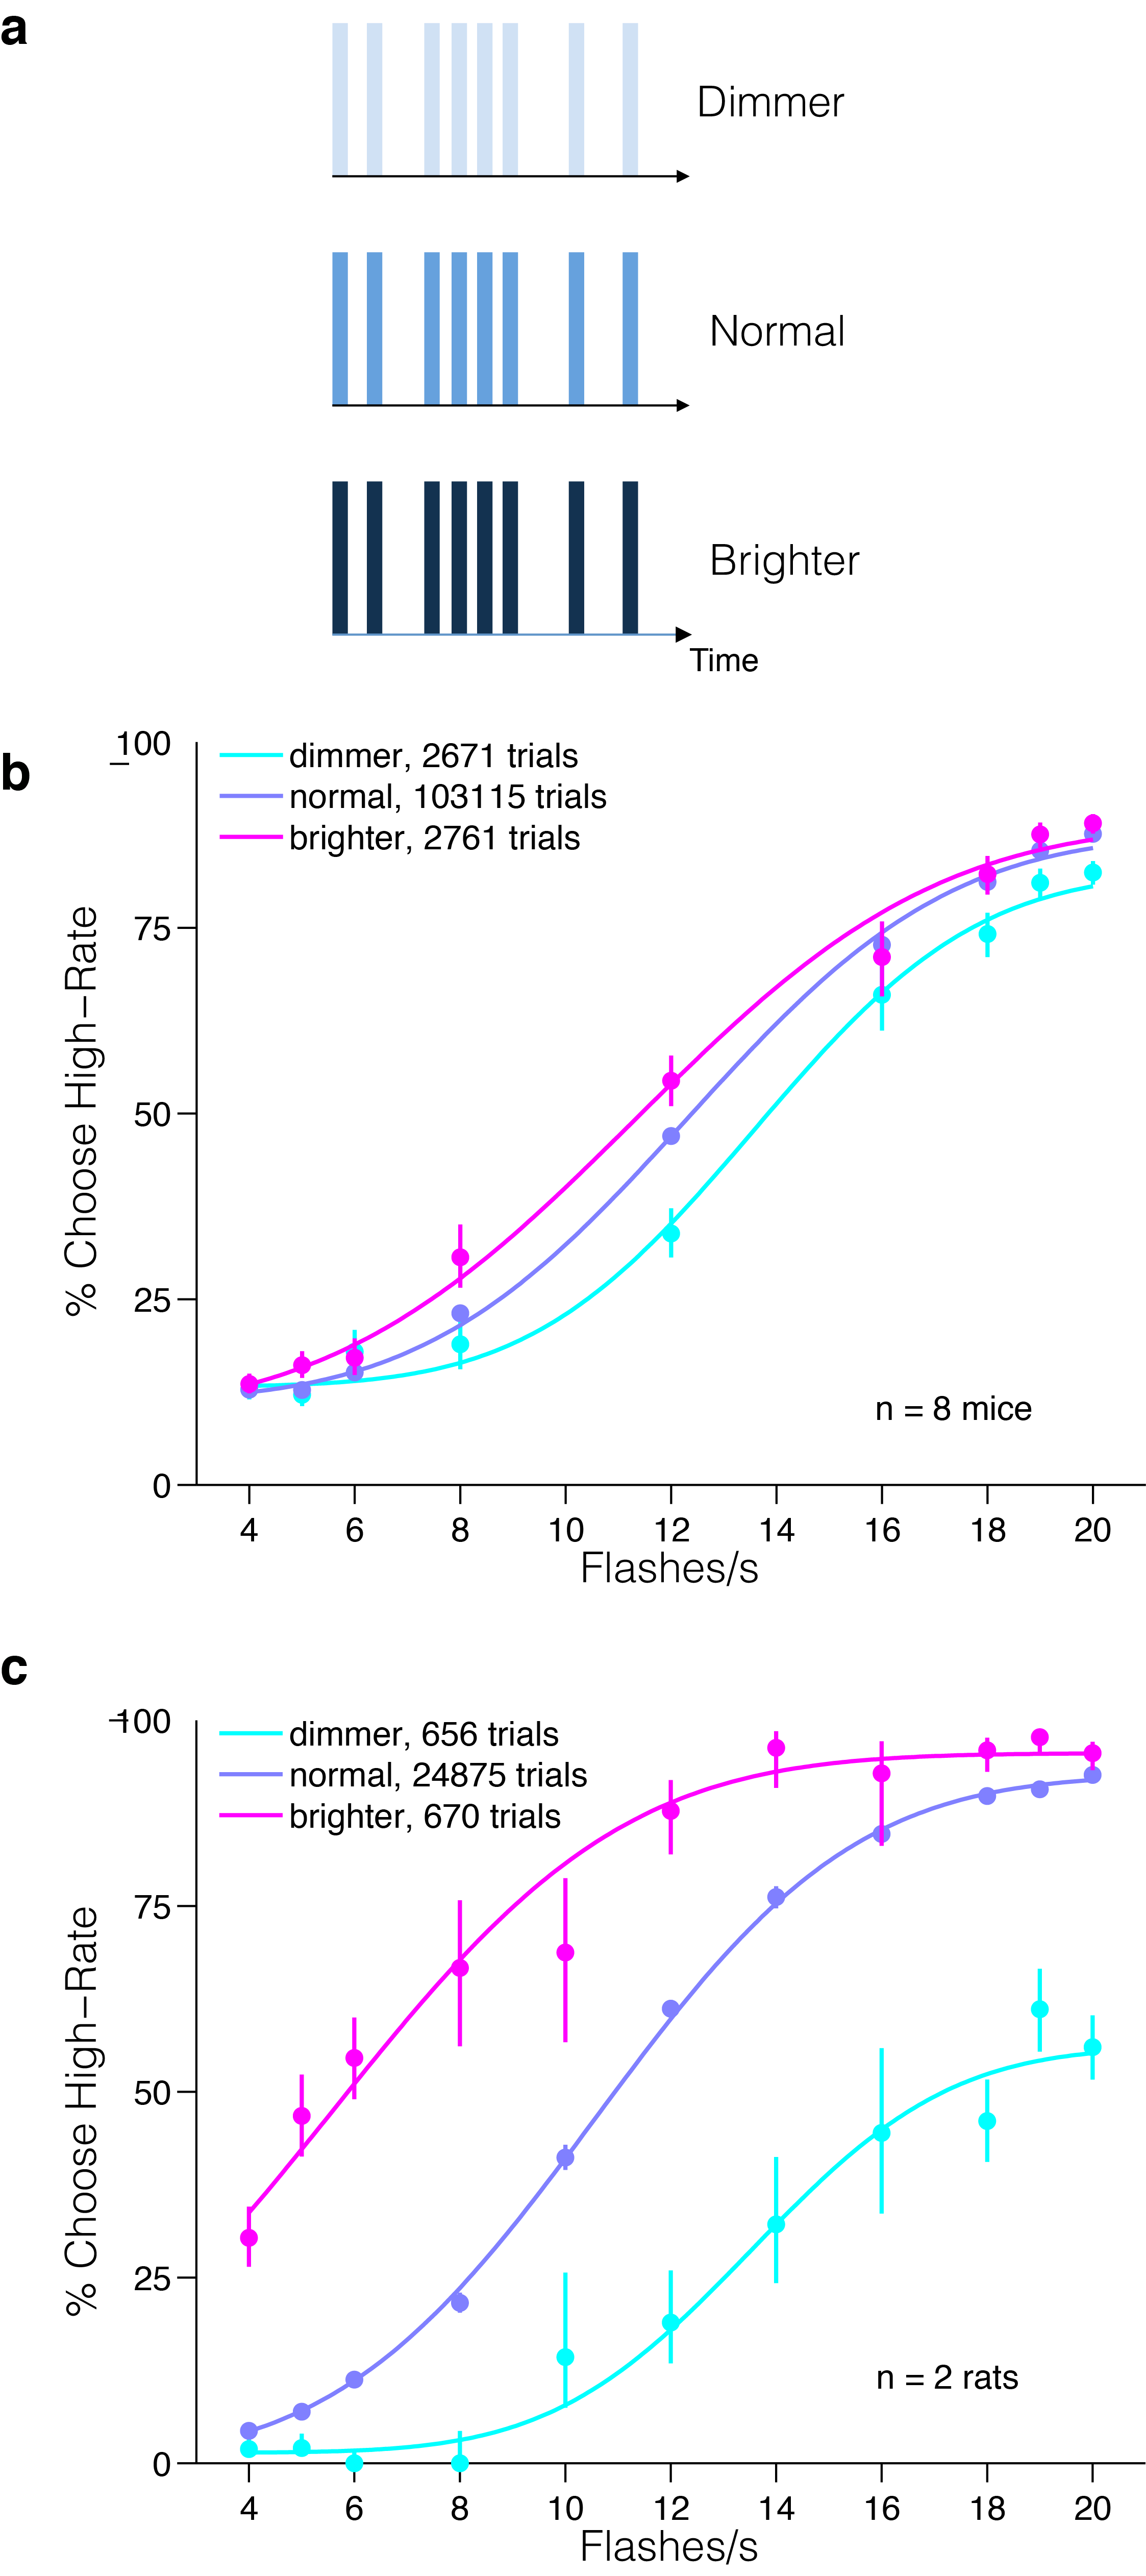
\includegraphics[width=\textwidth,height=0.8\textheight,keepaspectratio]{Figures/chapter2/brightness_manipulation_1.png}
  \caption[Brightness Manipulation Experiment 1]{\textbf{Brightness Manipulation Experiment 1}. (a) Schematic of random pulses sequence (8 flashes/s). The density of individual flashes were varied such that the flashes appeared dimmer or brighter than normal.(b) Mice (n = 8) or (c) rats (n=2) were presented with brighter (magenta) or dimmer (cyan) pulse sequences randomly on 5\% of trials. Circles represent subjects' behavioral response. Solid line represents 4-parameter cumulative Gaussian psychometric function fit to the data. Error bars represent Wilson binomial (95\%) confidence intervals.}
   \label{fig:brightness_exp1}
\end{figure}

\begin{figure}
  \centering
  	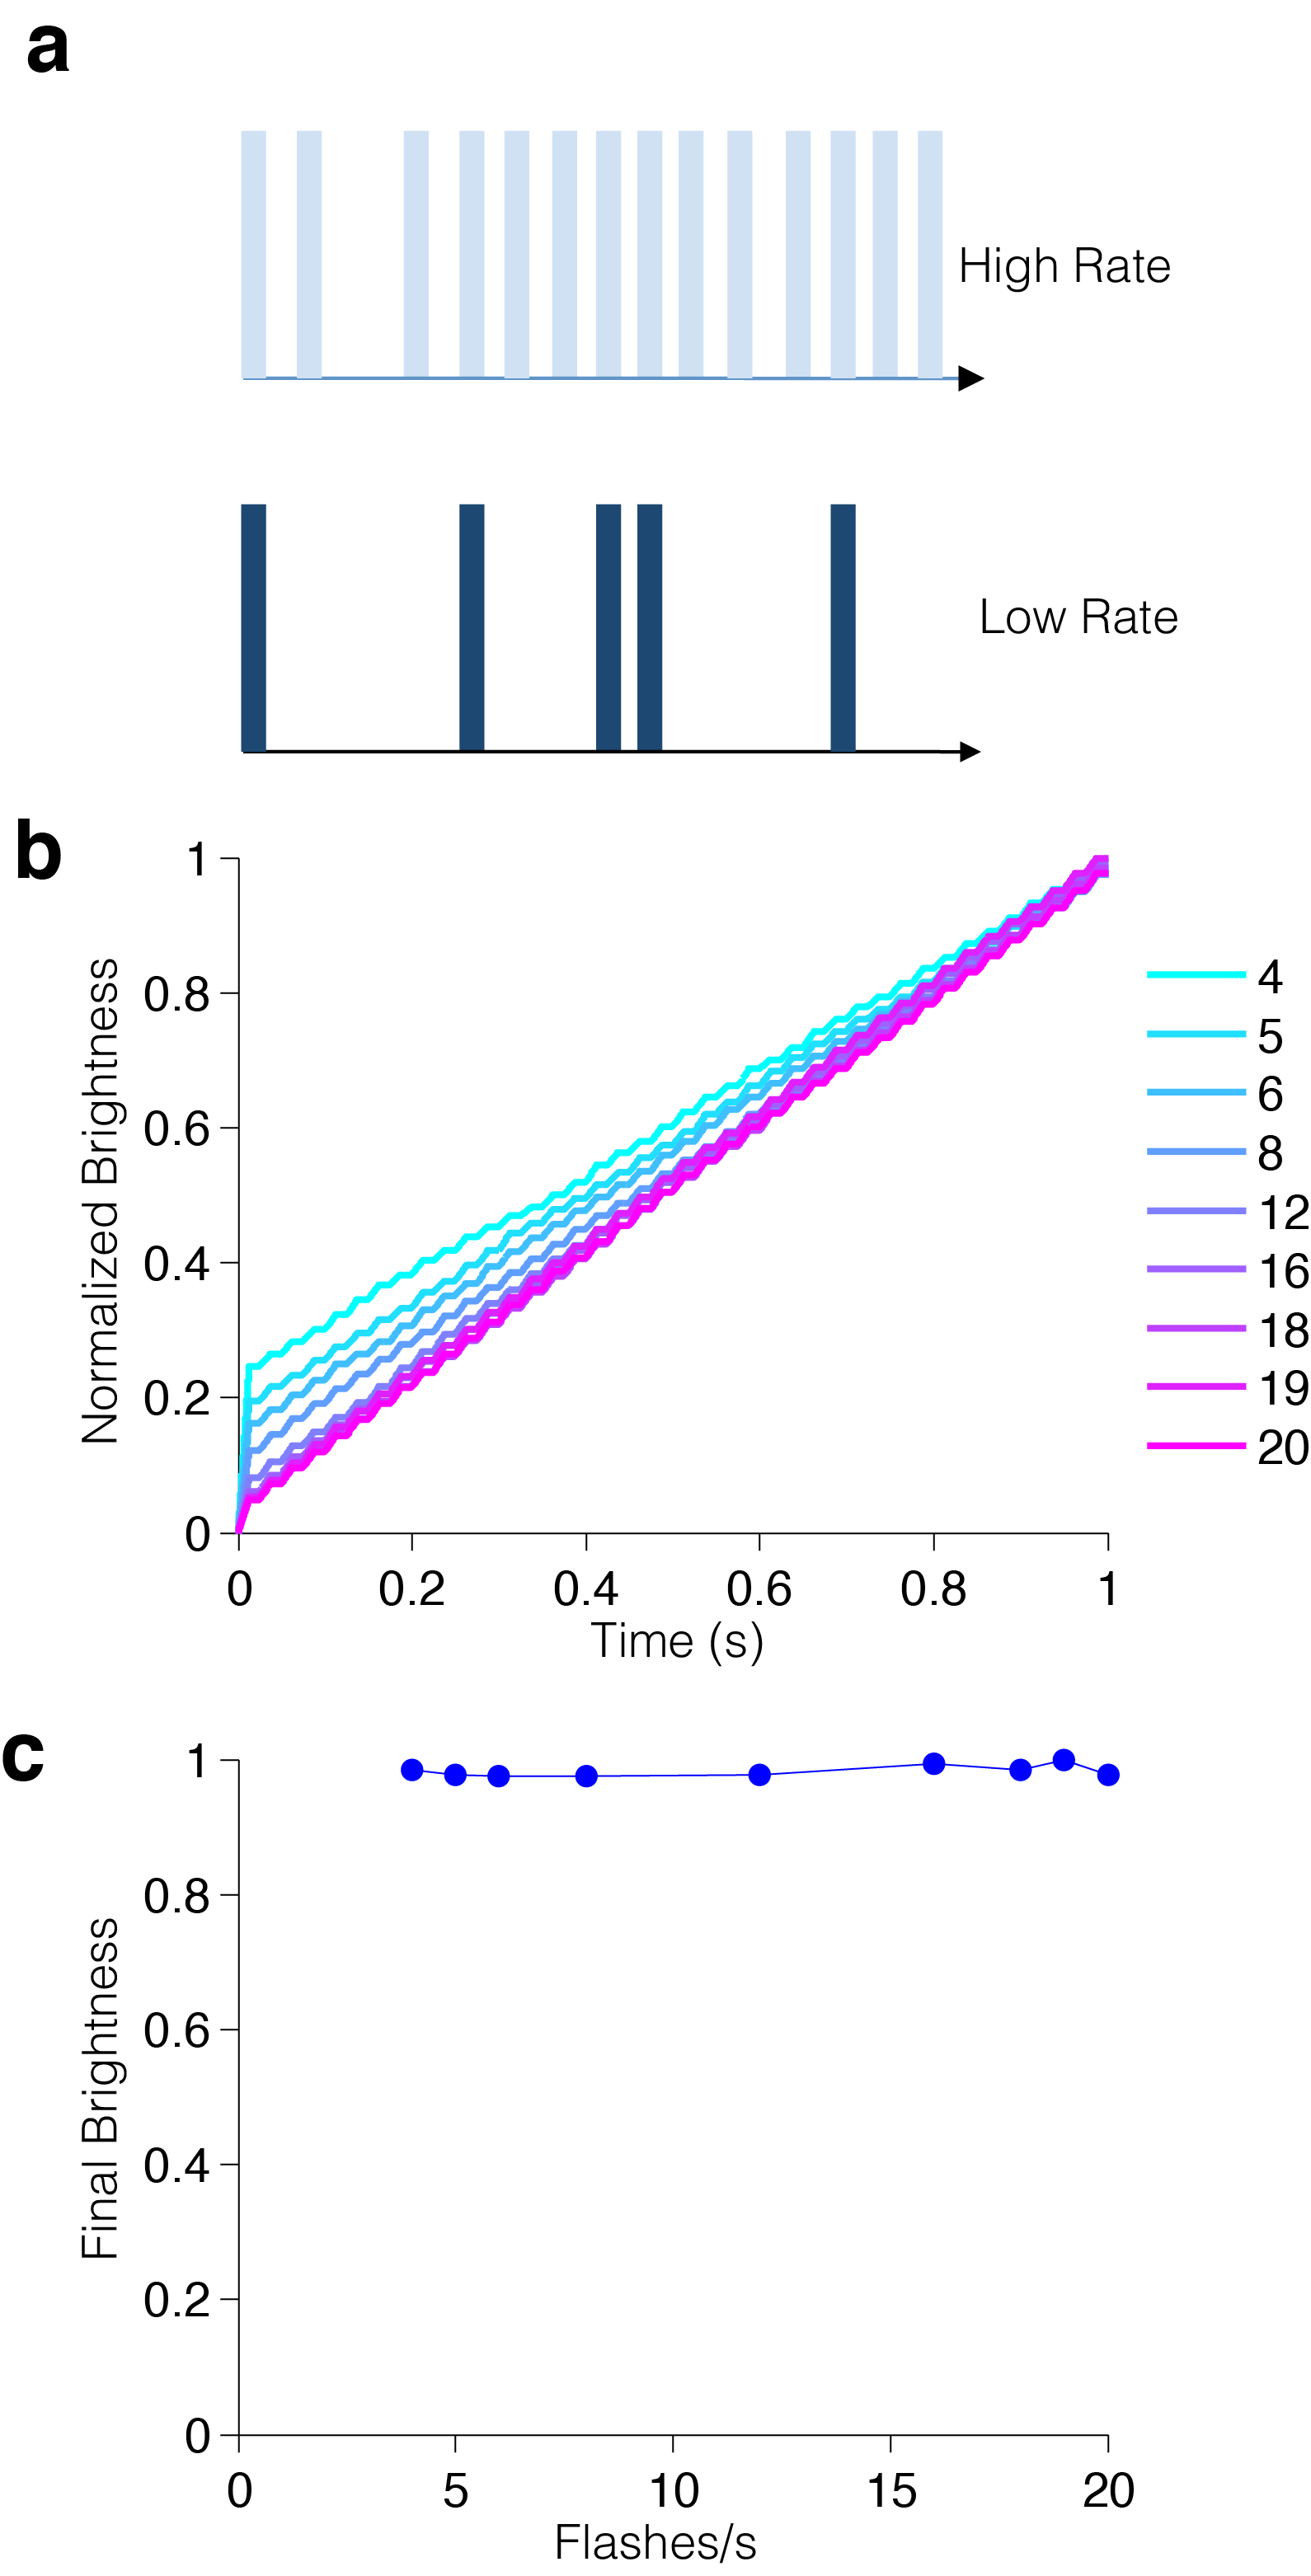
\includegraphics[width=\textwidth,height=0.8\textheight,keepaspectratio]{Figures/chapter2/brightness_simulation_scaled.png}
  \caption[Brightness Manipulation Experiment 2 Schematic]{\textbf{Brightness Manipulation Experiment 2 Schematic}. (a) Schematic of random pulses sequence for high-rate and low-rate example. The density of individual flashes are scaled inversely with the flash rate, such that the low-rate sequences are more dense than high-rate sequences. (b) Brightness over time is overlap for individual flash rate and (c) the final brightness value is equivalent across flash rates. }
   \label{fig:brightness_sim_man}
\end{figure}

\begin{figure}
  \centering
  	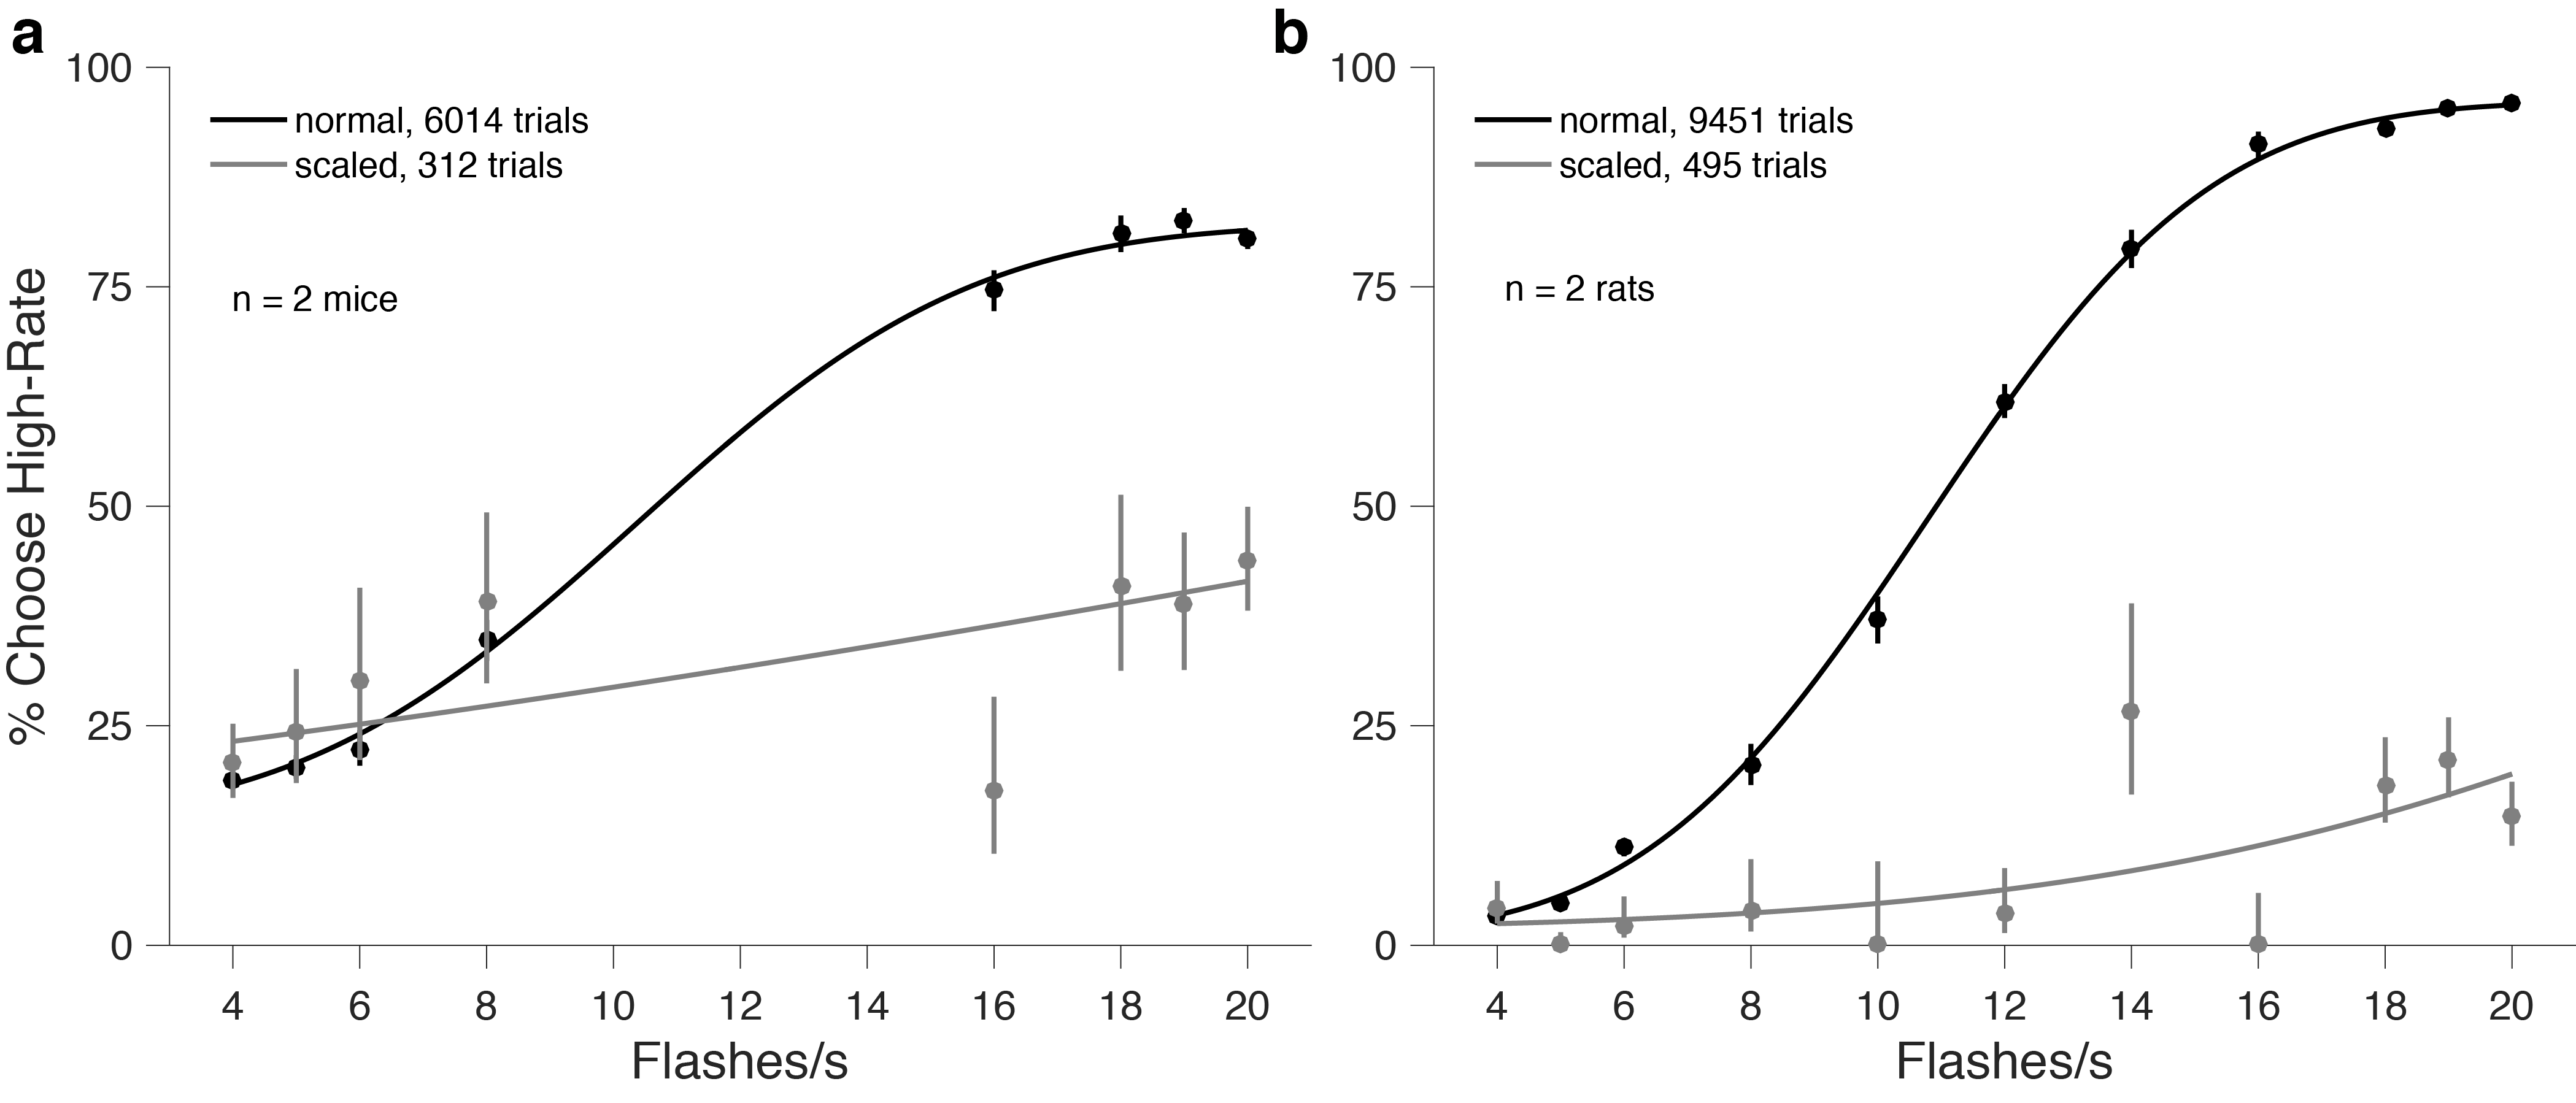
\includegraphics[width=\textwidth]{Figures/chapter2/brightness_manipulation_2.png}
  \caption[Brightness Manipulation Experiment 2]{\textbf{Brightness Manipulation Experiment 2}. (a) Mice or (b) rats were presented with the brightness scaled  pulse sequence randomly on 5\% of trials (open circle, gray curve). Circles represent subjects' behavioral response. Solid line represents 4-parameter cumulative Gaussian psychometric function fit to the data. Error bars represent Wilson binomial (95\%) confidence intervals. }
   \label{fig:brightness_exp2}
\end{figure}
%--------------------------------------------------------------------
\section{Previous Choice History Influence}
Several studies have found that both human and animal subjects performing perceptual tasks are influenced by previous choices \parencite{Busse2011,Frund2014,Scott2015SourcesRats,Abrahamyan2016,Urai2017}, even though the trials are independent and presented randomly. We used two quantitative models to assess whether mice trained to make categorical decisions about visual pulsatile stimuli were susceptible to choices made on previous trials.\par 
The first approach, assessed whether success or failure on the most recent trial influenced the performance on the current trial \parencite{Busse2011}: 
\begin{equation}
	\centering
	\ln(\frac{p_h}{1-p_h}) = \beta_0 + \beta_E E(t) + \beta_S I_{success} (t-1) + \beta_F I_{failure} (t-1)
    \label{eq:BusseChoice}
\end{equation}
where \emph{t} indicates the current trial and $\emph{E}$ is the signed stimulus evidence of the current trial. Evidence is computed as the difference between the flash rate of the trial and the category boundary (12 flashes/s). \emph{$I_{success}$} and \emph{$I_{failure}$} are indicator variables for success (reward) and failure on the previous trial, respectively. The coefficients ($\beta_0$,$\beta_E$,$\beta_S$,$\beta_F$) were estimated with MATLAB \emph{glmfit}.\par 
Figure \ref{fig:failsuccesshist} is a scatter plot of the coefficients for previous success, $\beta_S$, and previous failures, $\beta_F$. All mice (n = 27) had positive $\beta_S$ coefficients, indicating that mice tended to repeat the same choice on the current trial if they had been rewarded on the previous trial. Nearly half the group of mice had positive $\beta_F$ coefficients, meaning that these mice tended to repeat failures (Figure \ref{fig:failsuccesshist} , Stay quadrant). The remaining mice with negative $\beta_F$ coefficients had a tendency to switch choices if they were unsuccessful on the previous trials Figure \ref{fig:failsuccesshist}, (Win-Stay, Lose Switch quadrant). The observed trial history patterns are similar to those of human subjects performing a perceptual decision making task \parencite{Abrahamyan2016}. \par 
\begin{figure}
  \centering
  	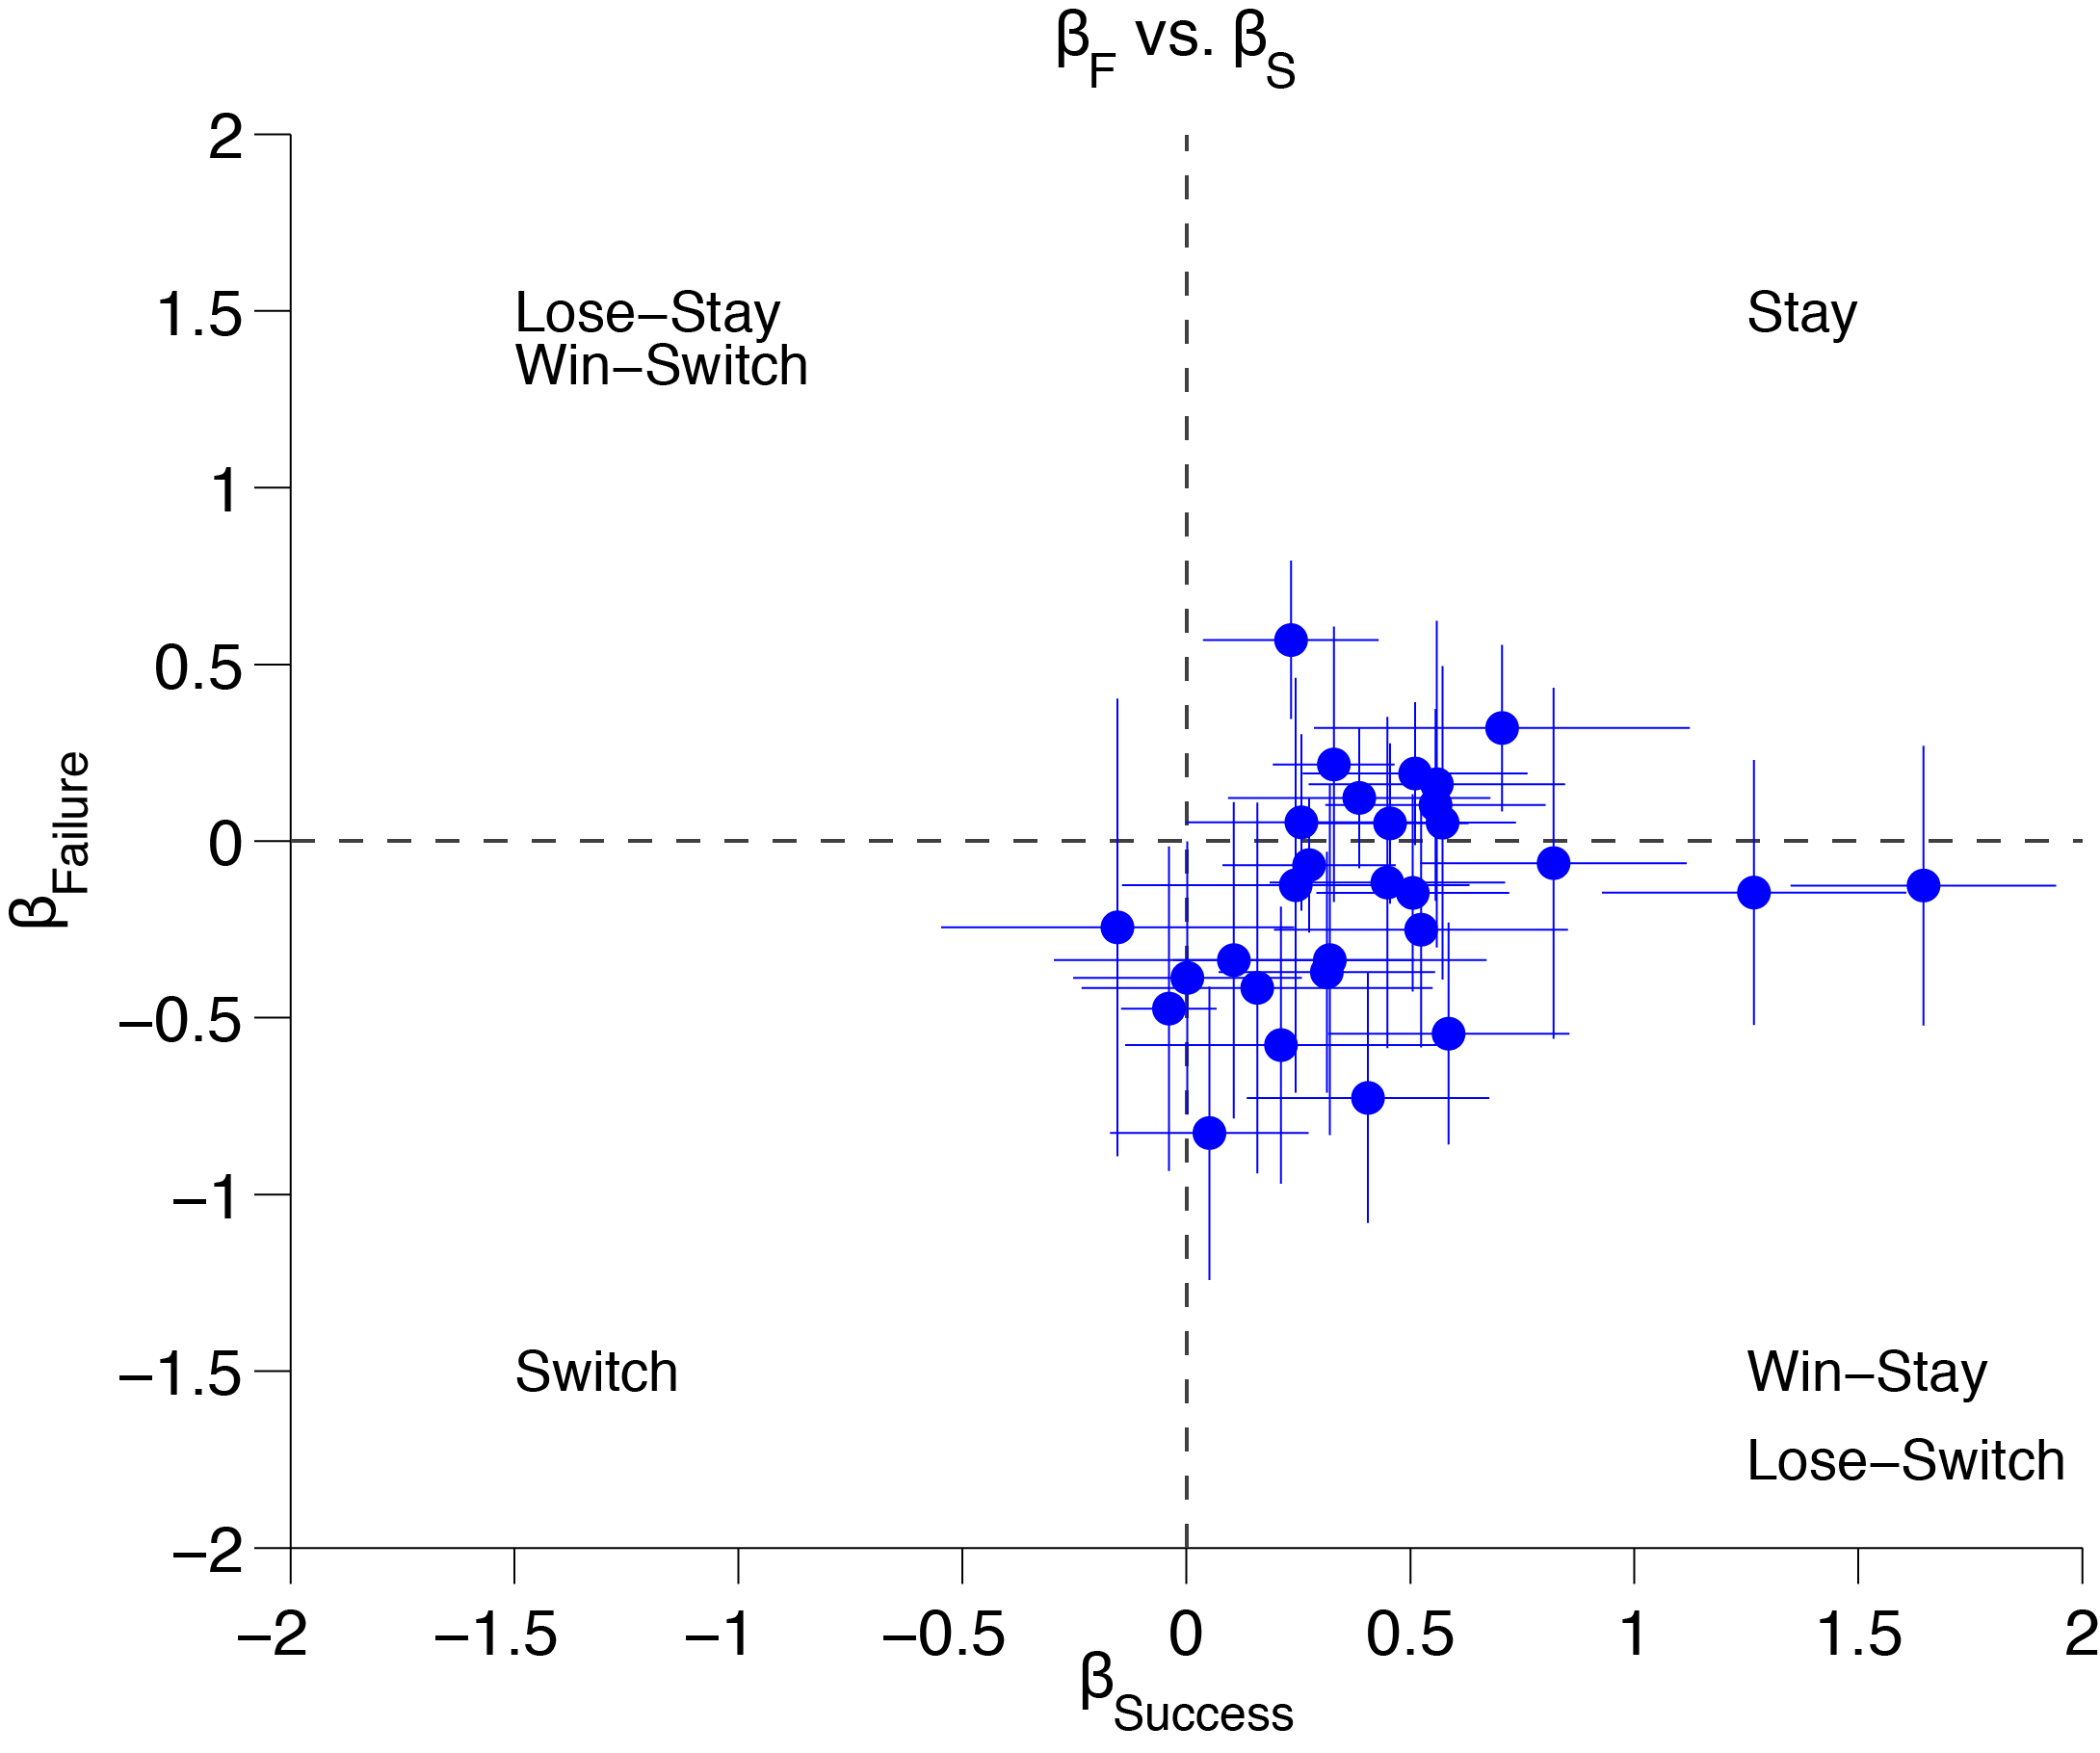
\includegraphics[width=\textwidth]{Figures/chapter2/history_failure_success_model_error_bars.png}
  \caption[Previous Choice History - Success and Failure]{\textbf{Previous Choice History - Success and Failure} Influence on the current trial for each mouse (n = 27 mice). Coefficients estimated for each session individually. Mean coefficients are plotted. Error bars represent standard error of the mean.}
   \label{fig:failsuccesshist}
\end{figure}
A second approach is to assess the influence of the history of previous choices on the current choice. The probabilistic model is an extension of Equation \ref{eq:BusseChoice} and equivalent to the model described in \textcite{Frund2014}:
\begin{equation}
	\centering
	\ln(\frac{p_h}{1-p_h}) = \beta_0 + \beta_E E(t) + \sum_{\tau = 1}^{T=7} \beta_{E(\tau)} E_\tau + \beta_{C(\tau)} C_\tau
\end{equation}
where \emph{t} indicates the current trial and  $\emph{E}$ is the signed stimulus evidence of the current trial. The additional regressors $E_\tau$ and $C_\tau$ represent the evidence and choice on $\tau$ previous trials in the past, respectively. Again, the coefficients ($\beta_0$,$\beta_E$,$\beta_{E(\tau)}$, and $\beta_{C(\tau)}$) were estimated with MATLAB \emph{glmfit}.\par 
\begin{figure}
  \centering
  	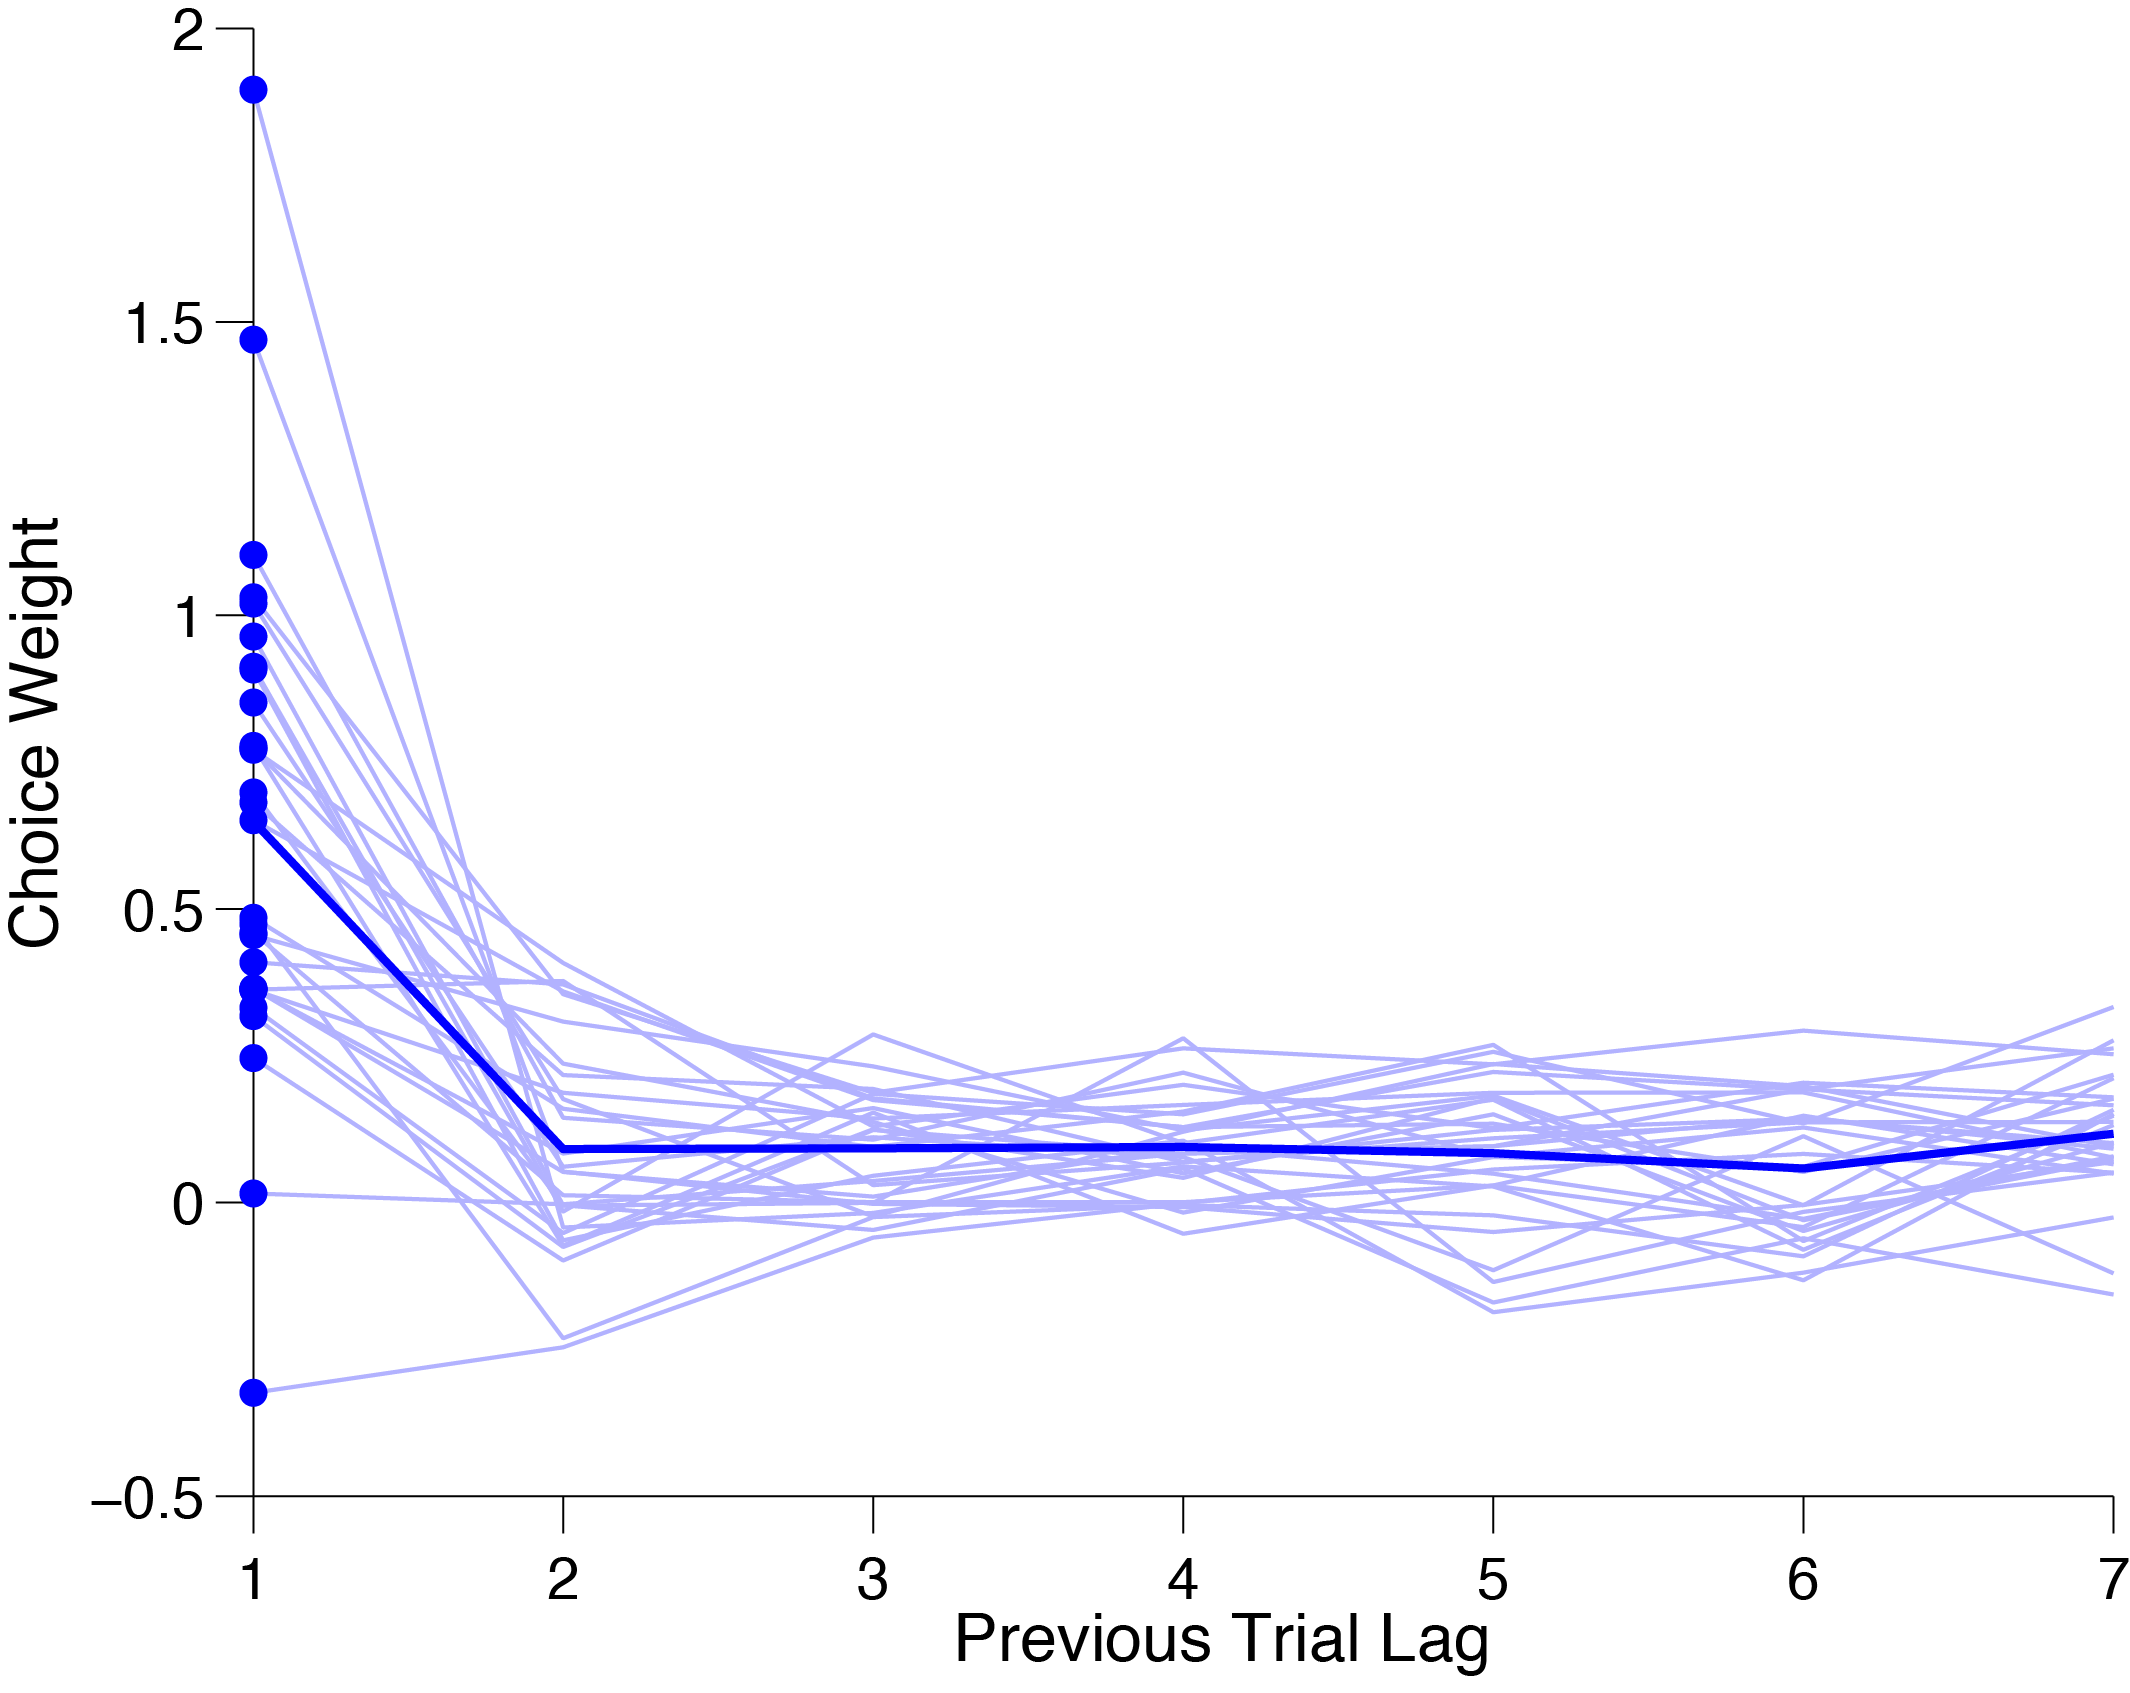
\includegraphics[width=\textwidth]{Figures/chapter2/history_past_choices_model.png}
  \caption[Influence of Previous Choice History]{\textbf{Influence of Previous Choice History} Choice weights, $\beta_{C(\tau)}$, associated with the previous seven trials. Light blue traces represent individual subjects (n = 27), Dark blue trace is the average across subjects.}
   \label{fig:prevchoiceshist}
\end{figure}
The model of the history of previous choices revealed that the most recent choice ($\tau$ = 1) had a greater influence on the choice of the current trial, than all other trials in the past (Figure \ref{fig:prevchoiceshist}). Almost all the subjects exhibited the same trend. 
%----------------------------------------------------------------------------
\section{Behavioral Correlates of Decision Uncertainty}
Response time is inversely correlated with decision certainty (i.e. confidence) \parencite{Kiani2014,Sanders2016,Urai2017}. I evaluated whether the response times of the mice trained on the visual pulses task exhibited the three signatures of decision uncertainty, the complement of the decision confidence \parencite{Kepecs2008,Sanders2016,Urai2017}, which make the following predictions: (1) accuracy monotonically decreases with uncertainty (Figure \ref{fig:uncertainty}a), (2) average uncertainty decreases with evidence strength for correct choices and increases for incorrect choices (Figure \ref{fig:uncertainty}b), and lastly, for fixed evidence strengths, low and high uncertainty change the slope of the psychometric function (Figure \ref{fig:uncertainty}c). \par 
Although the mice were trained to perform the task under fixed duration (or interrogation) protocol \parencite{Bogacz2006}, we measured a proxy of reaction time as the time it takes the mice to exit the center port and enter the side reward port. A similar approach was used in a recent study by \textcite{Urai2017} to correlate response time of human subjects performing a fixed duration perceptual decision-making task.\par 
\begin{figure}
  \centering
  	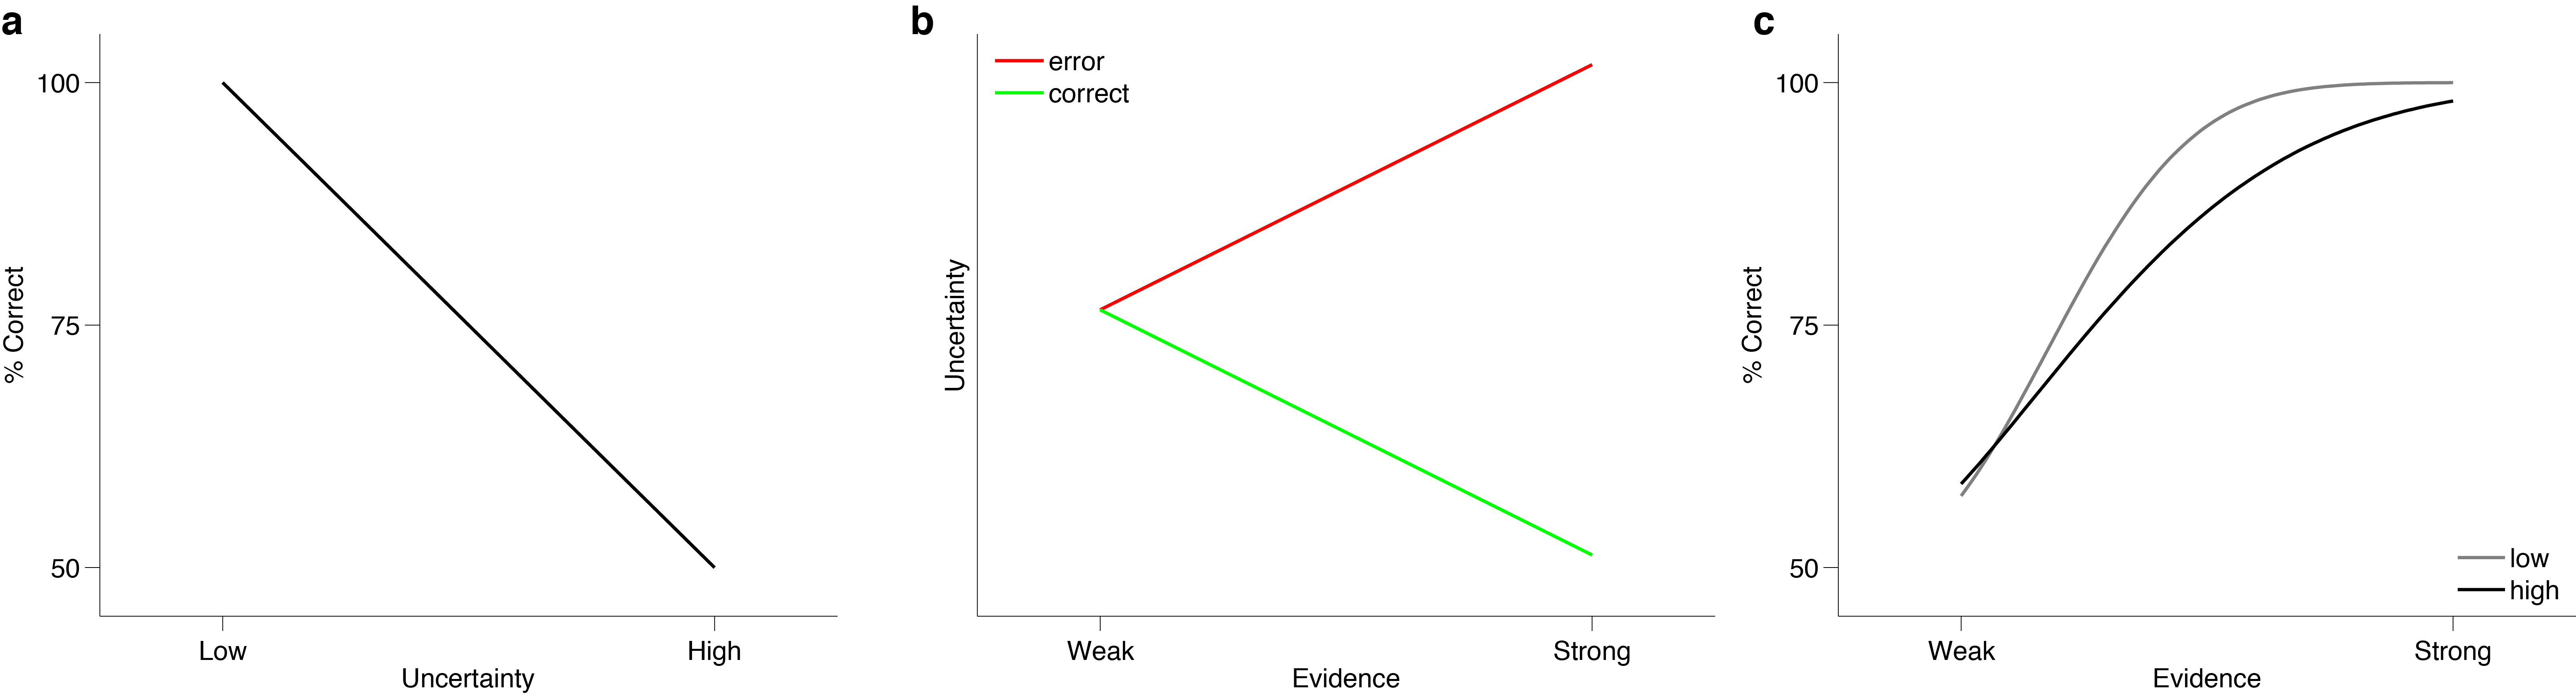
\includegraphics[width=\textwidth]{Figures/chapter2/schematic_uncertainty_predictions.png}
  \caption[Schematic of Signatures of Decision Uncertainty Predictions]{\textbf{Schematic of Decision Uncertainty Predictions} (a) Monotonic decrease in accuracy with uncertainty Scaling of accuracy (b) Scaling of mean uncertainty with evidence strength for correct (green) and incorrect (red) choices (c) Psychometric function predictions for low (gray) and high uncertainty (gray). Adapted from \textcite{Urai2017,Sanders2016}}
   \label{fig:uncertainty}
\end{figure}
For the following analyses we evaluated mice trained under two different conditions. One group of mice (n = 10) were trained with walls between the center port and the side ports and the second group were trained without the walls (n = 19 mice) and rewarded in the center (0.5 $\mu$L) for waiting the minimum required wait duration. The group trained with walls were trained before we implemented the center reward approach (Figure \ref{fig:completeRate}). In the early stages of the thesis project, walls were used to reduce the subjects' impulsive tendencies to break center fixation and respond to the side port. The walls also helped to make the subjects' movements more stereotyped across animals. However, when trained mice were tethered with optical fibers for optogenetic stimulation (or microdrives for neural recordings), the walls obstructed the subjects' movements, so we removed the walls entirely from the training protocol.\par 
\begin{figure}
  \centering
  	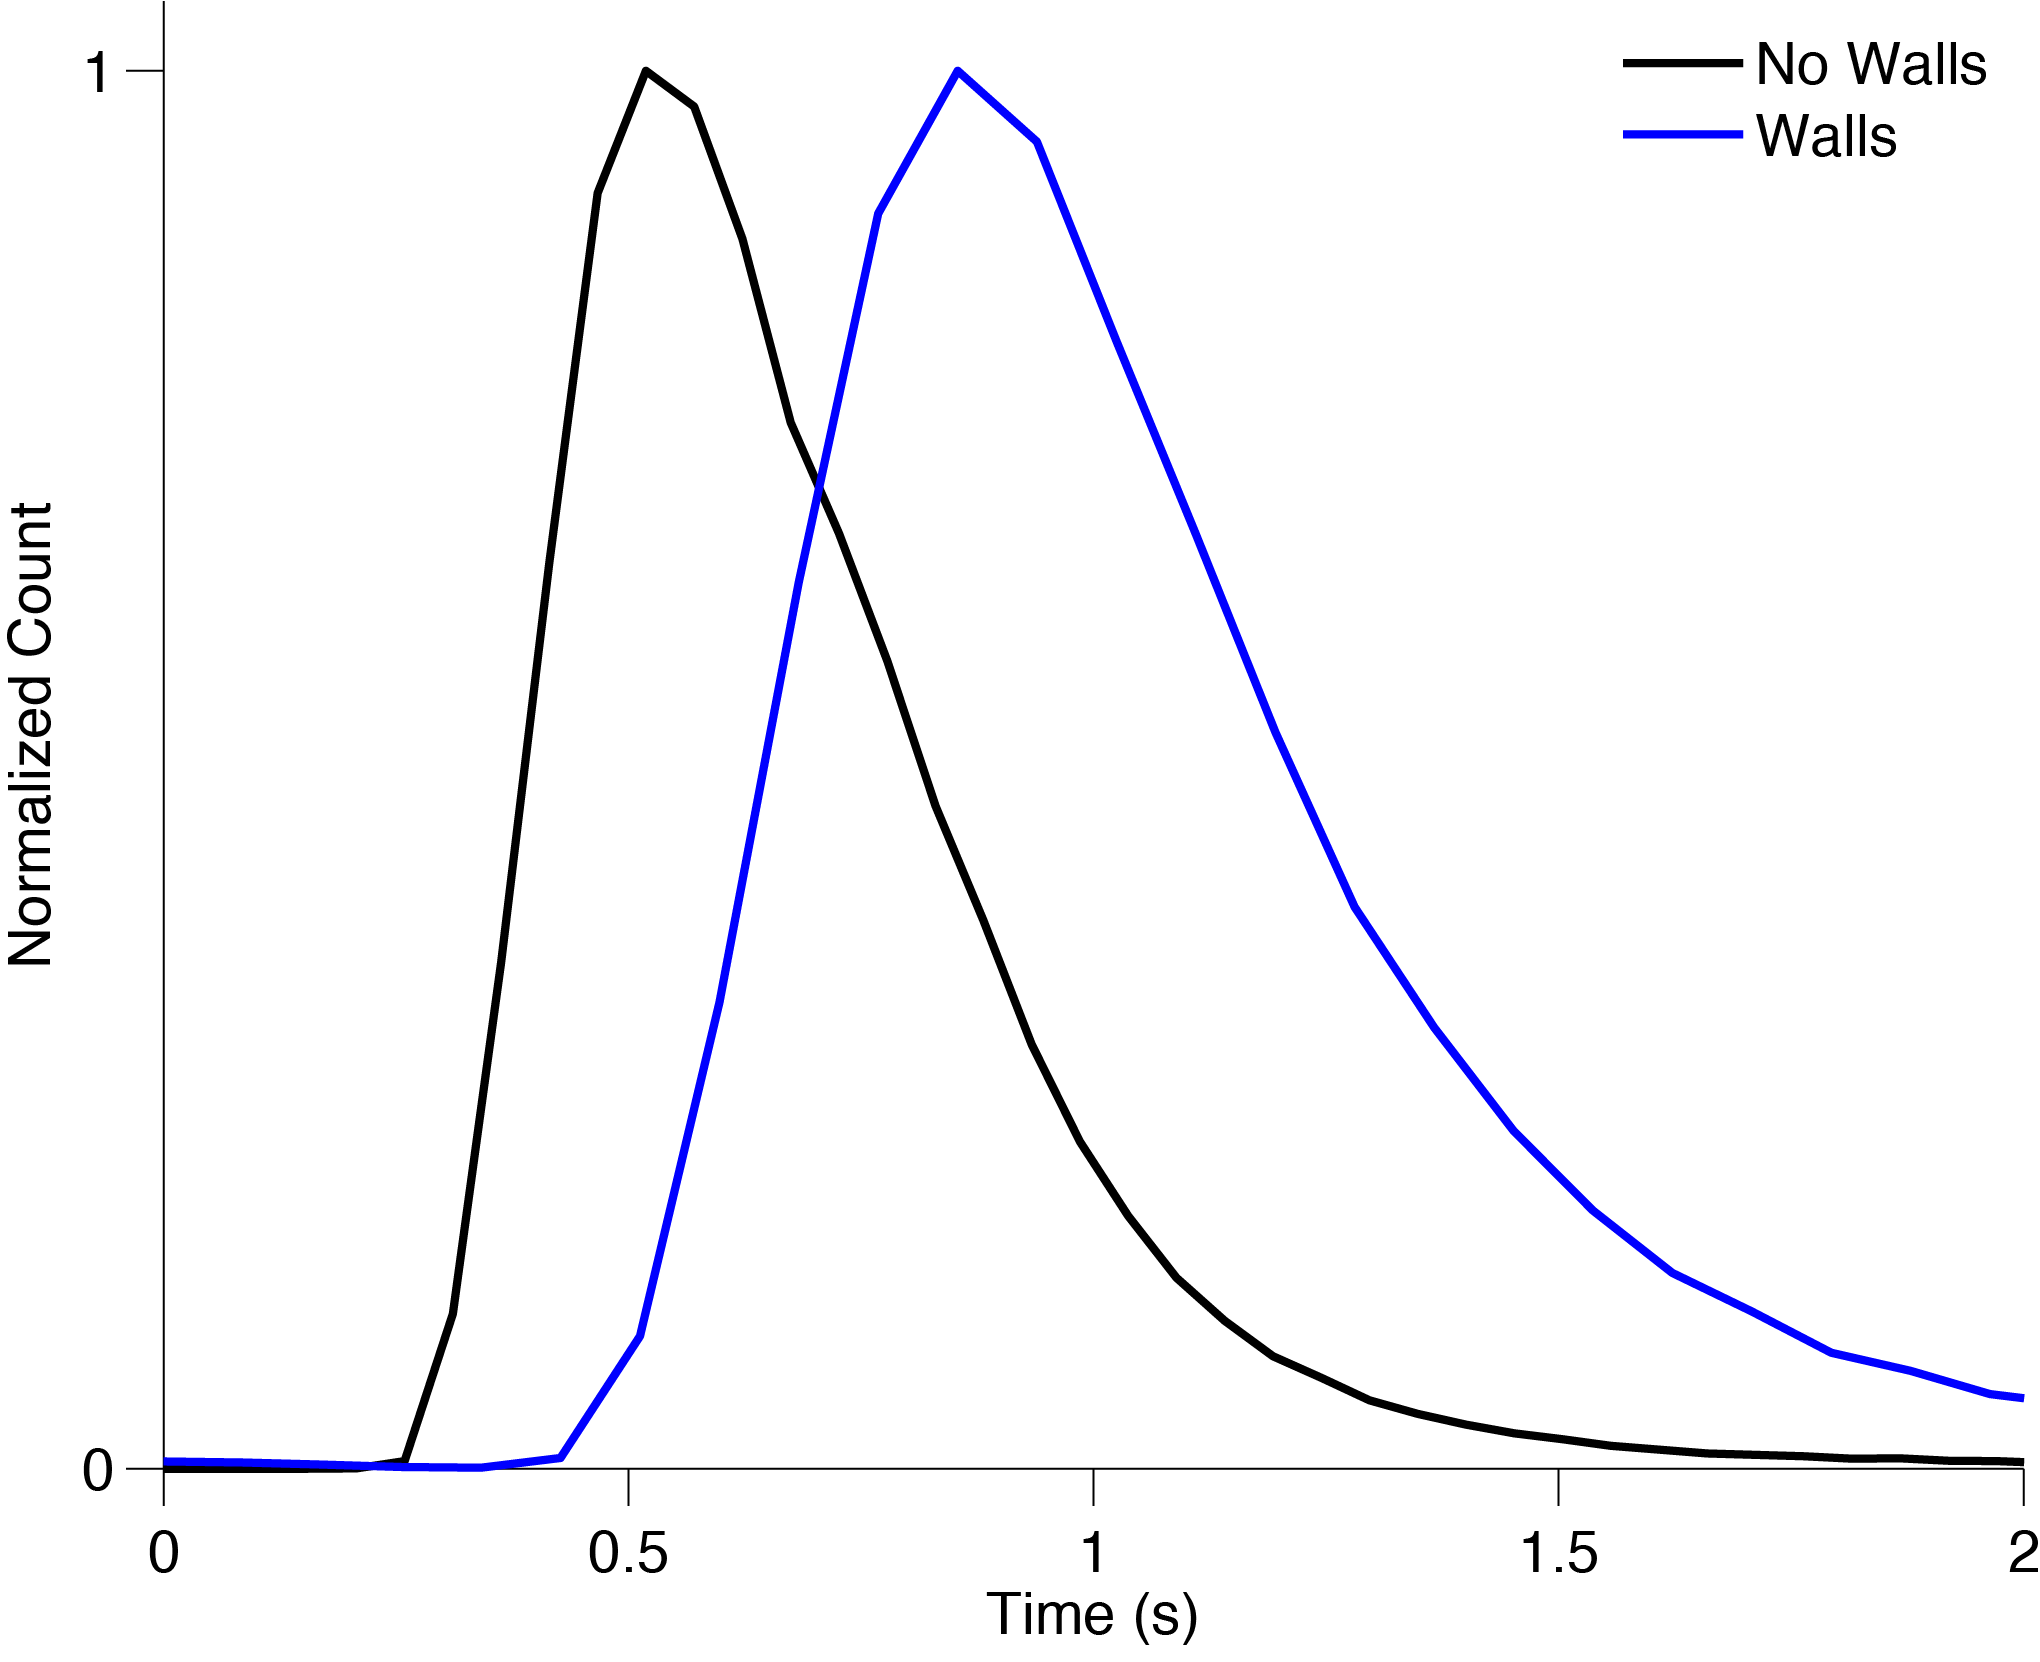
\includegraphics[width=\textwidth]{Figures/chapter2/RTHistogram_Combined.png}
  \caption[Response Time Histogram]{\textbf{Response Time Histogram} For mice trained with walls (blue, n = 10 mice) and without walls (black, n = 19 mice)}
   \label{fig:rthistogram}
\end{figure}
Mice trained with walls took much longer to reach the side reward ports than mice trained without the walls (Figure \ref{fig:rthistogram}). Similar to \textcite{Urai2017} we used the response time as our proxy for decision uncertainty. Surprisingly, there were differences in the uncertainty signatures between the two groups (Figures \ref{fig:rtuncertainty}). Response times from the mice trained with walls mirrored all three predictions of decision uncertainty (Figure \ref{fig:rtuncertainty} a-c). The performance accuracy decreased monotonically with response time (Spearman's correlation, $\rho$ = -1, p-value = 0.0167) (Figure \ref{fig:rtuncertainty}a). The mice responded more quickly on correct trials and responded more slowly on incorrect trials with increasing evidence strength  (Figure \ref{fig:rtuncertainty} b). Sensory evidence was calculated as the absolute difference between the flash rate and and the category boundary (12 flashes/s). Also, performance accuracy was greater on trials with higher response times (Figure \ref{fig:rtuncertainty} c). However, the response times from the second group of mice that were trained without walls and with an additional center reward did not recapitulate the predictions of decision uncertainty (Figure \ref{fig:uncertainty} d-f). \par 
\begin{figure}
  \centering
  	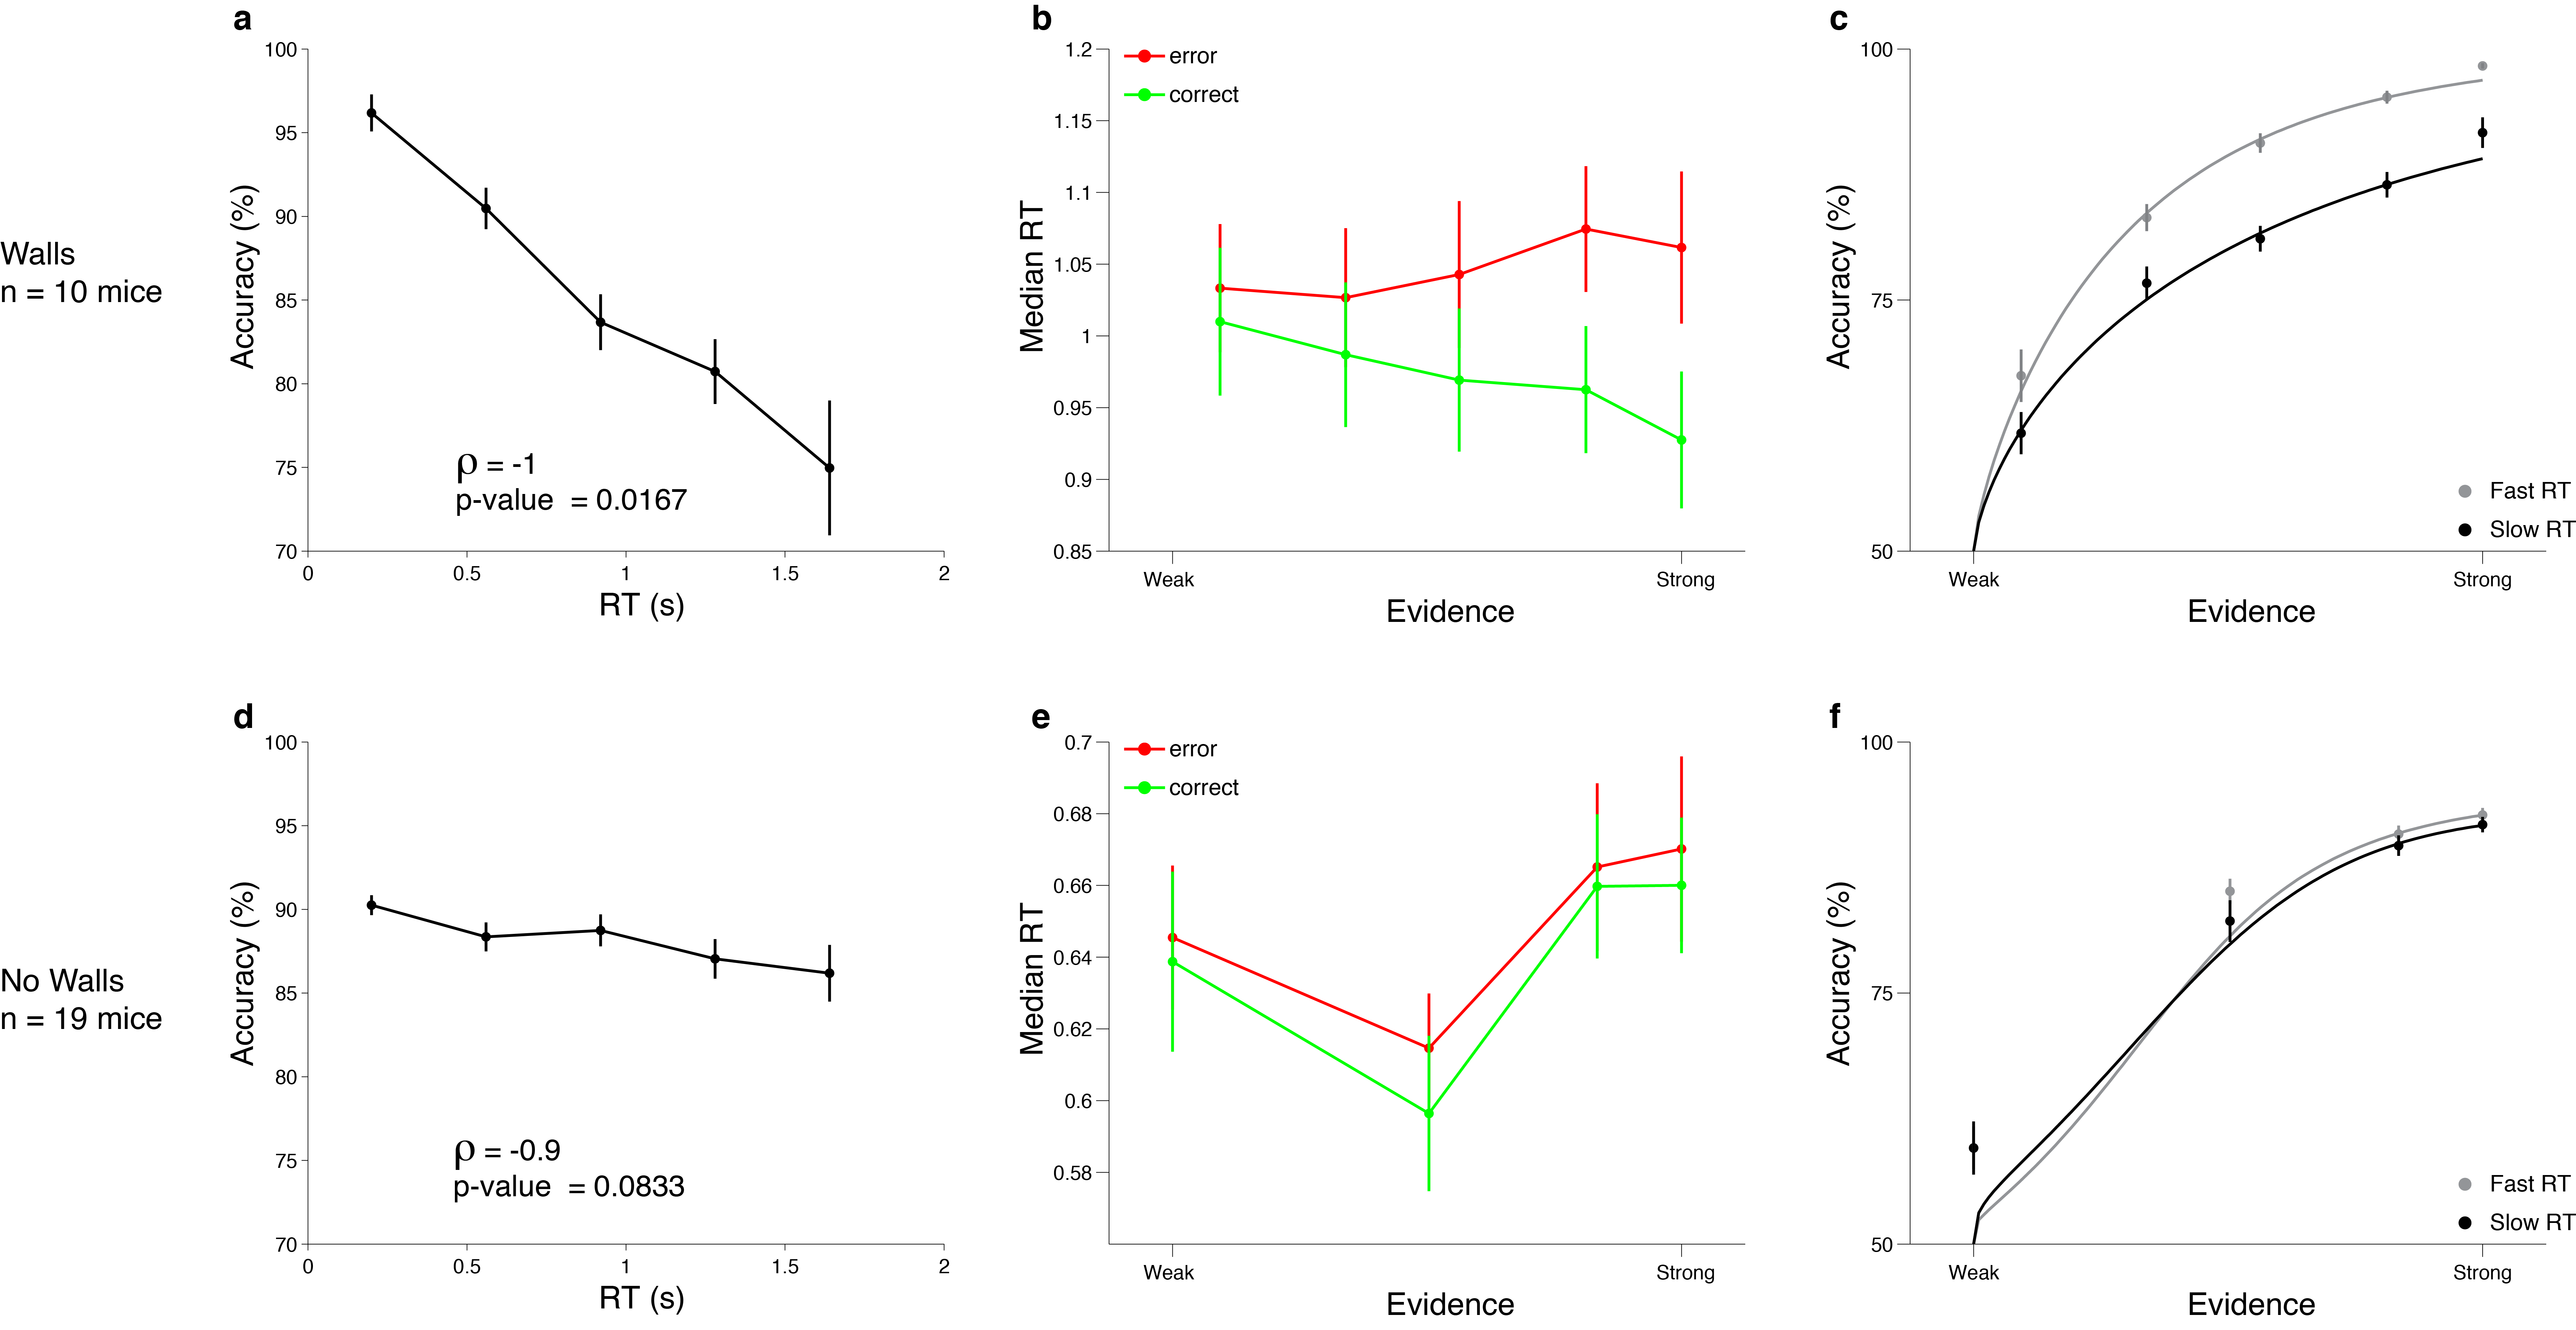
\includegraphics[width=\textwidth]{Figures/chapter2/RTUncertaintySignatures.png}
  \caption[Response Time and Decision Accuracy]{\textbf{Response Time and Decision Accuracy} Response time measured as the total time from Go-cue to side reward port. (First Row) Trained with walls n = 10 mice (Second Row) Trained without walls n = 19 mice. (a, d) Percent correct as a function of binned response times. (b,e) Median response time as a function of absolute sensory evidence. (c,f) Psychometric function for fast and slow response times. Error bars are SEM.}
   \label{fig:rtuncertainty}
\end{figure}
One explanation for the differences between the two groups is that signatures of perceptual uncertainty is associated with the cost to act. For the mice trained with walls, the cost is associated with moving around the physical barrier to the reward port. Hence, when the mouse is certain, they respond rapidly, and when uncertain it is more likely to guess. However, mice trained without the walls do not incur an additional movement and time cost in reaching towards the reward port. The cost, however, is associated with leaving the center port where they are also rewarded for waiting. Thus, the mice in this second group are more likely to spend less  time at the center port after the Go-cue when they are certain, and in most cases forgo the additional small center reward (0.5 $\mu$L) for the the larger side reward (2 $\mu$L). Conversely, when uncertainty is high the mouse will spend more time at the center port, harvesting the small center reward (the sure bet). To examine whether the three uncertainty signatures are present when response time is measured as additional time spent at the center port, I repeated the analyses in Figure \ref{fig:rtuncertainty} for the mice trained without walls. In Figure \ref{fig:rtuncertaintyNoWalls} a, the decision accuracy decreases monotonically with the additional time spent in the center (Spearman's correlation $\rho$=-1, p-value = 0.0833), consistent with the prediction that mice may forgo the small center reward when uncertainty is low and conversely spend more time harvesting the center reward when uncertainty is high. There was no difference between response time scaling with evidence for correct and error trials (Figure \ref{fig:rtuncertaintyNoWalls} b). However, accuracy was slightly higher for fast response times than slow response times (Figure \ref{fig:rtuncertaintyNoWalls} c).\par 
\begin{figure}
  \centering
  	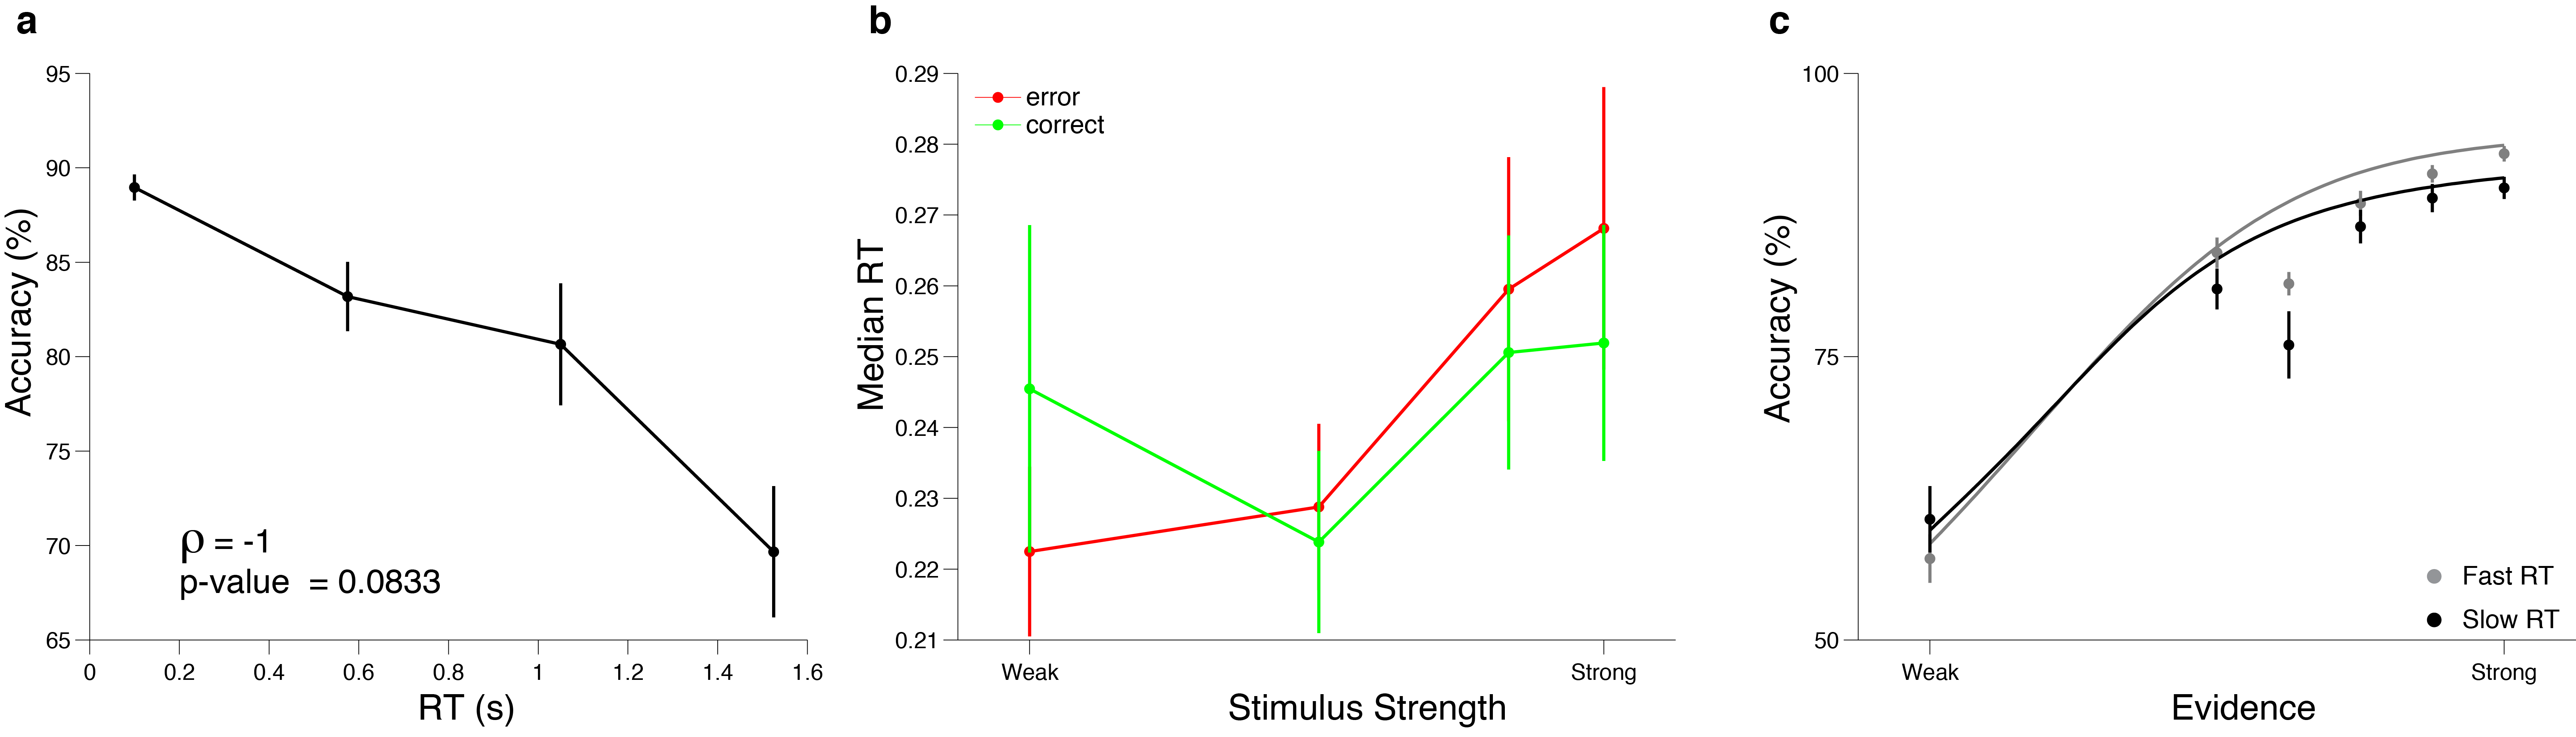
\includegraphics[width=\textwidth]{Figures/chapter2/RTUncertaintySignaturesNoWallsExtraCenter.png}
  \caption[Response Time and Decision Accuracy-No Walls]{\textbf{Response Time and Decision Accuracy} Response time measured as the additional time spent in the center port from Go-cue for mice trained without walls n = 19. (a) Percent correct as a function of binned response times. (b) Median response time as a function of absolute sensory evidence. (c) Psychometric function for fast and slow response times. Error bars are SEM.}
   \label{fig:rtuncertaintyNoWalls}
\end{figure}
These results indicate that for the mice trained without the walls and rewarded in the center, response time does not fully account for perceptual uncertainty as previously suggested by \textcite{Sanders2016}. With the current data, it is not clear whether the presence of the walls or the center liquid reward led to the presence or absence of signatures of behavioral uncertainty. An interesting experiment would be to directly test whether behavioral correlates of decision uncertainty are associated with the cost to act. One such way to test this with the current paradigm is to train mice with walls and reward in the center. Further, the center reward can be delivered on all trials or on a fraction of "catch" trials. \par 

\section{Discussion}
The focus of this chapter has been to provide a quantitative description of the behavior of mice performing an accumulation of visual evidence task. Such quantitative descriptions are important for generating and constraining mechanistic models of evidence accumulation. In the task, mice are presented with a rich stimulus set which allows them to explore and generalize across the stimulus space. Mice perform several hundreds of trials per session and maintain stable performance across sessions. In solving the task, the mice tend to deviate from an ideal strategy, whereby on average more weight was assigned to pulses presented earlier in trial, reflecting a snap judgment strategy. Similar to previous perceptual studies in humans and animals, mice trained on this paradigm were influenced by previous reward and choice history, further lending evidence that reward history is a source of behavioral variability or noise in visual evidence accumulation \parencite{Scott2015SourcesRats}. Lastly, the response times of mice trained with walls capture the signatures of decision uncertainty, whereas response times from mice trained without walls and rewarded in the center do not fully account for decision uncertainty. The difference in the two groups of mice suggests that the signatures of decision uncertainty might be influenced by the cost to act. 



